\documentclass[hidelinks,12pt]{article}

\usepackage[brazil]{babel}
\usepackage[utf8]{inputenc}
\usepackage{amsmath}
\usepackage{amsfonts}
\usepackage{amssymb}
\usepackage{indentfirst}
\usepackage{color}
\usepackage{mathrsfs}
\usepackage{pgfplots}
\usepackage{hyperref}
\usepackage{fancyhdr}
\usepackage[export]{adjustbox}
\newcommand{\icon}[1]{\includegraphics[height=12pt]{#1}}
\newcommand{\bigicon}[1]{\includegraphics[height=50pt]{#1}}

\newcommand{\iconb}[1]{\includegraphics[height=20pt]{#1}}
\setcounter{secnumdepth}{5}

\fancypagestyle{plain}{%
	\fancyfoot{}%
	\fancyhead{}%
}


\begin{document}
\pagenumbering{gobble}
\pagestyle{fancy}


\lhead{\bigicon{Figures/ufu}}
\chead{{\footnotesize UNIVERSIDADE FEDERAL DE UBERLÂNDIA \\ FACULDADE DE CIÊNCIA DA COMPUTAÇÃO \\ COMPPET - PROGRAMA DE EDUCAÇÃO TUTORIAL} \\ \scriptsize{Av. João Naves de Ávila 2121, Campus Santa Mônica} }
\rhead{\bigicon{Figures/facom}}
\lfoot{}
\cfoot{}
\rfoot{}
\vspace*{1cm}
\begin{figure}[!h]
	\centering
	
\includegraphics[scale=0.18]{Figures/capa.png}
\end{figure}


\newpage
\fancyhead[C]{}
\fancyhead[R]{\iconb{Figures/comppet}}
\fancyhead[L]{\leftmark}
\fancyfoot{}
\fancyfoot[L]{{\footnotesize  COMPPET - Programa de Educação Tutorial}}
\fancyfoot[C]{\hspace{3.0cm}\thepage}
\fancyfoot[R]{{\footnotesize Curso de Inclusão Digital}}
\pagenumbering{arabic}


\tableofcontents
\listoffigures

{\let\thefootnote\relax\footnotetext{* \textit{COMPPET - UFU, Universidade Federal de Uberlândia, Minas Gerais, Brasil}}}

{\let\thefootnote\relax\footnotetext{* \textit{PETMEC - UFU, Universidade Federal de Uberlândia, Minas Gerais, Brasil}}}

{\let\thefootnote\relax\footnotetext{* \textit{PETCIVIL - UFU, Universidade Federal de Uberlândia, Minas Gerais, Brasil}}}

\newpage

\section{Introdução}

 Este material foi desenvolvido por alunos do PET-Computação, PET-Eng. Civil, PET-Eng. Mecânica da UFU (Universidade Federal de Uberlândia) e visa, prioritariamente, ajudar aqueles que tiveram pouco, ou nenhum, contato com o computador e o nicho no qual ele está inserido. Nas primeiras partes, você aprenderá tarefas simples como ligar e desligar o computador; utilizar mouse e teclado; utilizar o sistema operacional (Windows 7). Depois, mostraremos como editar um texto e como utilizar a Internet.
 
 Ao final do curso, você será capaz de entender como um computador funciona e como usá-lo. Contudo, o que mais esperamos que você aprenda é conseguir buscar novos conhecimentos pelo computador, pois mesmo se este curso durasse 6 meses, não seriamos capazes de ensinar tudo que é possível de se realizar com um computador. Assim, espero que goste e qualquer sugestão é sempre bem vinda. \textbf{Enfim, chega de papo e vamos ao que realmente interessa!!!}


\section{Ligando e Desligando o Computador}
\label{Ligando e Desligando o Computador}

\subsection{Ligando o Computador}
\label{Ligando o Computador}

	
Para ligar o computador, devemos seguir os seguintes passos:
	
\begin{enumerate}
	\item Ligar o \textbf{estabilizador}, caso exista. Ele possui um botão Liga/Desliga e, na maioria das vezes, possui também uma ``luz'' indicando se já está ligado. Assim, quando o botão for acionado, a luz do estabilizador deve acender;

	\item Ligar o computador através do botão Liga/Desliga, localizado no \textbf{gabinete}. Sempre que o computador estiver ligado, espera-se que se possa ouvir barulhos e ver luzes vindas do gabinete;

    \item Ligar o Monitor, caso ele ainda não esteja ligado;

	\item Aguardar, com paciência, até que apareça no Monitor a \emph{tela inicial};

	\item Informar senha e nome do usuário, caso existam e quando for solicitado.
\end{enumerate}


\subsubsection{Verificando configurações de energia}

Caso for a \textbf{primeira vez que o seu computador será ligado}, e você não tiver nenhuma pessoa mais experiente te ajudando, é necessário tomar alguns cuidados antes de ligá-lo:

\begin{itemize}
    \item Verificar os cabos de energia do computador;
    
    \item Verificar se a voltagem está correta (110 volts ou 220 volts);
    
    \item Verificar se existe um estabilizador de voltagem, e se existir, verificar a voltagem dele (110 v ou 220 v). Essa voltagem deve ser compatível com a voltagem utilizada no local onde você irá ligar o aparelho;
    \textbf{OBS}.: notebooks modernos geralmente acompanham uma bateria bivolt. Dessa forma pode-se ligá-los em qualquer lugar, sem preocupação.
\end{itemize}


\subsection{Desligando o Computador}
\label{Desligando o Computador}

O procedimento de desligar o computador é muito importante para preservar o equipamento e as informações armazenadas nele, portanto, é importantíssimo acostumar-se a seguir o procedimento de desligar:

\begin{enumerate}
	\item Clicar no botão Iniciar;

	\item Clicar na opção Desligar;

	\item Esperar o computador finalizar o desligamento. Você saberá que esse passo terminou quando não houver mais nenhum barulho ou luz vindo do gabinete. Além disso, o monitor mostrará uma tela preta.

	\item Desligar o estabilizador através do botão Liga/Desliga do estabilizador.
\end{enumerate}

\begin{figure}[!h]
	\centering
	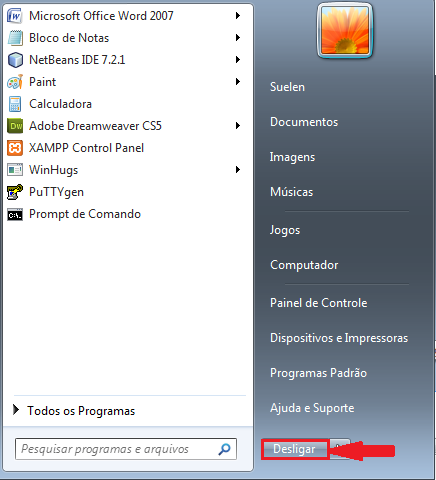
\includegraphics[scale=0.9]{Figures/desligando.png}
	\caption{Desligando o Computador}
	\label{fig:desligando}
\end{figure}

\newpage

\section{Comunicando com o computador}
\label{Comunicando com o computador}


Agora que já aprendemos a ligar o computador, precisamos interagir com ele; pedir a ele o que desejamos. A principal forma de se comunicar com o computador é por meio do \textbf{Mouse} e do \textbf{Teclado}. E a principal forma dele se comunicar com a gente é pelo \textbf{Monitor}.

Se você ainda não está familiarizado com os dispositivos acima, fique tranquilo; falaremos um pouco de cada um agora. E saiba que se acostumar com eles requer tempo. No começo, pode parecer muito estranho e complicado, mas logo logo estará acostumado a utilizá-los.

\subsection{Mouse}
\label{Mouse}


\begin{figure}[!h]
	\centering
	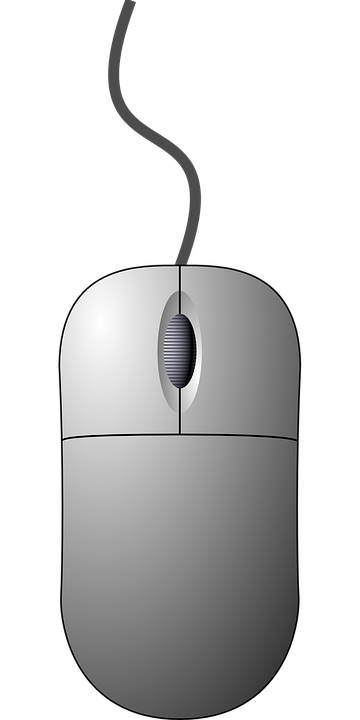
\includegraphics[scale=0.2]{Figures/mouse}
	\caption{Um de vários exemplos de Mouse}
	\label{fig:mouse}
\end{figure}

O mouse é como se fosse o nosso dedo indicador para o computador. Com o mouse você consegue ``apontar'' para o computador as coisas que você deseja realizar. Se quiser saber para onde você está ``apontando'' nesse exato momento, basta olhar para a ``setinha'' que deve estar na sua tela. Essa ``setinha'' é mais comumente chamada de \textbf{ponteiro}. O ponteiro anda pelo monitor de acordo com a forma que você movimenta o mouse. 

\subsubsection{Ponteiros}

Como falado anteriormente, o ponteiro te permite visualizar para onde você está apontando. No entanto, ele também pode te dar algumas outras informações dependendo da forma com que ele está desenhado.


\begin{figure}[!h]
	\centering
	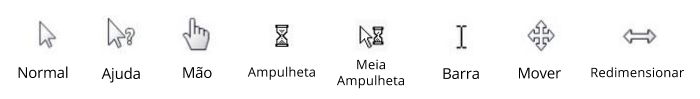
\includegraphics[width=\textwidth]{Figures/ponteiros}
	\caption{Tipos de Ponteiro}
	\label{fig:ponteiros}
\end{figure}


\begin{itemize}
	\item \textbf{Normal}: é assim que o ponteiro fica durante a maior parte do tempo. Ela não te passa nenhuma informação adicional.
	
	\item \textbf{Ajuda}: O ponto de interrogação significa que você pode obter ajuda para alguma ação. Deixe o mouse quieto alguns segundos e o texto de ajuda relacionado é exibido.
	
	\item \textbf{Ampulheta}: mostra que o computador está fazendo muito esforço ``pensando'', e por isso as coisas que você estiver fazendo podem parecer devagar. É recomendado esperar um pouco até que a ampulheta desapareça.
	
	\item \textbf{Ampulheta com seta branca}: indica que o computador está ``pensando''/``trabalhando'', mas com menor intensidade. Nesse estado, não é necessário dar um tempo pro computador, pode continuar normalmente a utilizá-lo.
	
	\item \textbf{Barra} : indica que o lugar em questão é um local de ``textos''. Assim, ela permite \emph{selecionar um texto}, ou \emph{ativar o funcionamento do teclado} (fazendo aparecer um \emph{cursor}).
	
	\item \textbf{Mão}: é muito usado na internet (\emph{links}) e aparece quando você está sobre um elemento clicável. Lembre-se: \textbf{se a mão aparecer, basta clicar uma vez, não duas}. Além disso, quando o ponteiro estiver nessa forma, se você deixar o mouse parado durante alguns instantes, aparecerá uma pequena frase falando algo sobre o elemento.
	
	\item \textbf{Mover}: as flechas apontadas para quatro direções servem para avisar que você pode \emph{mover o elemento} que está por baixo mantendo o botão esquerdo pressionado e movendo o mouse;
	
	\item \textbf{Redimensionar}: as flechas opostas são usadas para \emph{mudar o tamanho} das coisas. Elas geralmente aparecem nos cantos das janelas.

\end{itemize}

\subsubsection{Botões do Mouse}
\label{botoes-mouse}

Vimos então que o ponteiro na tela do computador segue o movimento do mouse. No entanto, o computador só realmente percebe que você está apontando para um lugar e \emph{querendo fazer alguma coisa} quando você utiliza um dos \textbf{botões} do mouse.

O ato de \emph{apertar e soltar} um botão do mouse é chamado de \textbf{clicar}. Assim, quando pedirem para \emph{clicar} em algum lugar, estão na verdade pedindo: \emph{mova} o ponteiro do mouse até aquele lugar e \emph{aperte e solte} o botão correspondente (geralmente o botão esquerdo).

O mouse possui pelo menos três botões:

\begin{figure}[!h]
	\centering
	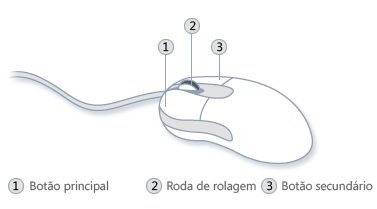
\includegraphics{Figures/mouse-botoes}
	\caption{Botões de um Mouse}
	\label{fig:mouse-botoes}
\end{figure}

\begin{itemize}
	\item \textbf{Botão Esquerdo}: é o botão principal. Ele possui diversas funcionalidades, as quais dependem da forma de se clicar esse botão:
	
	\begin{itemize}
	    \item \textbf{Clique Normal}: você aperta e solta o botão esquerdo uma única vez. Ele serve para selecionar coisas e abrir links.
	    
	    \item \textbf{Clique Duplo}: acotece quando você aperta e solta o botão esquerdo \emph{duas vezes seguidas}. Leva um tempo para se acostumar com esse tipo de clique, pois os dois cliques precisam ser rapidinhos. Ele é utilizado para \emph{abrir} coisas.
	    
	    \item \textbf{Arraste}: você \emph{aperta e continua pressionado} (não solta) o botão , enquanto que movimenta o mouse. Isso faz com que o computador entenda que você vai selecionar várias coisas ao mesmo tempo. Assim, enquanto estiver segurando o botão, você selecionará todas as coisas por onde o seu ponteiro passar.
	\end{itemize}
	
	\item \textbf{Botão Direito}: ele é o botão ``coringa''. É utilizado quando se quiser saber as várias ações que podem ser feitas no lugar clicado. Assim, quando apertado, abre-se uma \emph{janela} com as possiveís opções.
	
	\item \textbf{Botão Central ou Rodinha}: nem sempre todas as coisas que o computador quer te mostrar cabem na tela, assim, a rodinha serve para dizer ao computador que você gostaria de ver mais coisas, ou voltar para as coisas que você já viu. A rodinha pode ser entendida como uma manivela que faz a tela do computador ir para baixo ou para cima.
\end{itemize}


\subsubsection{Mouse para Canhotos}

Como você deve ter percebido, o mouse está previamente configurado para ser utilizado por pessoas destras. Mas caso você seja canhoto (possui mais coordenação motora com a mão esquerda) não perca o ânimo; tem como fazer ele funcionar naturalmente para os canhotos. Consulte um dos ministrantes para mais informações.

\subsection{Teclado}
\label{Teclado}


\begin{figure}[!h]
    \centering
	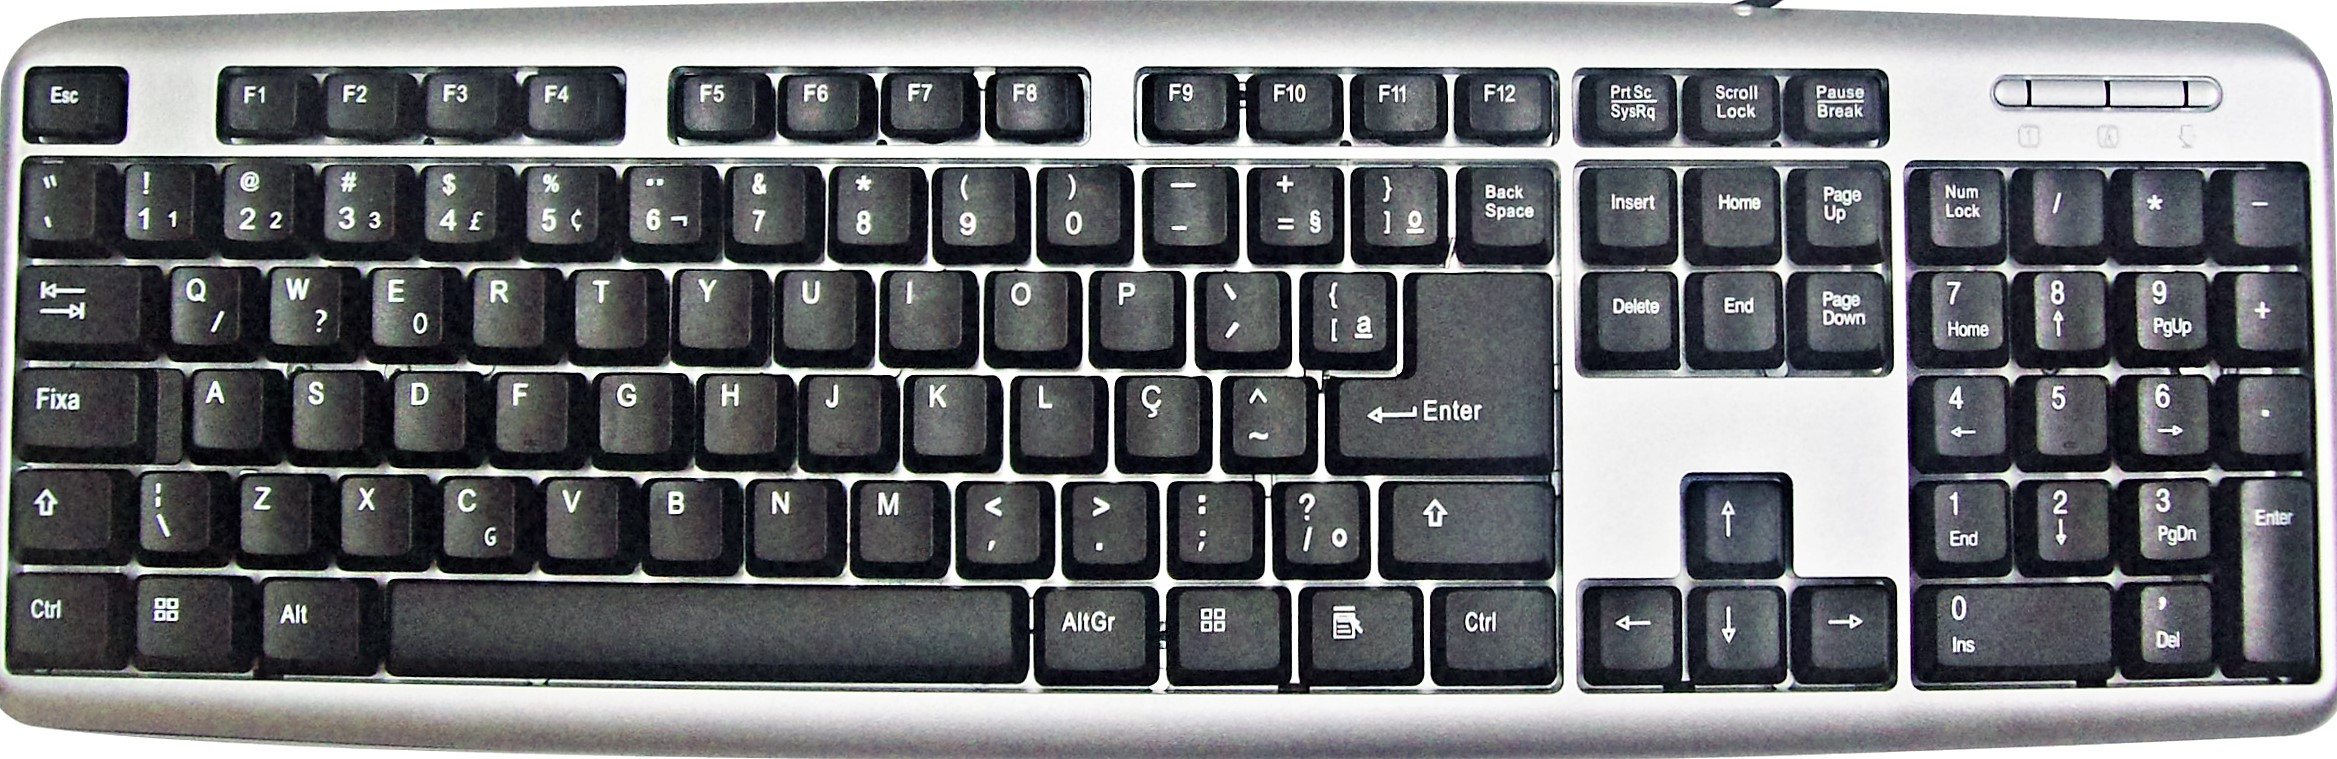
\includegraphics[scale=1]{Figures/teclado}
	\label{fig:teclado}
	\caption{Exemplo de um Teclado}
\end{figure}

É por meio do teclado que podemos ``escrever'' palavras e textos no computador, mas, assim como uma máquina de escrever, ele possui também diversas teclas especiais que permitem ir muito além da escrita. 

O ato de ``escrever'' por meio de um teclado é chamado de \textbf{digitação}. Um detalhe importante na hora de digitar é saber se o computador está realmente pronto para receber o que você estiver digitando. Assim como o mouse possui um ponteiro na tela para mostar aonde você está apontando, o teclado possui um \textbf{cursor} (\emph{barra}). Entâo, \emph{sempre que você ver uma barrinha piscando na tela, saiba que o computador receberá o que você estiver digitando naquele exato lugar}.

\begin{figure}[!h]
    \centering
	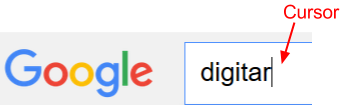
\includegraphics[scale=0.7]{Figures/cursor1}
	\label{fig:cursor1}
	\caption{Cursor esperando para receber algo digitado}
\end{figure}

\begin{figure}[!h]
        \centering
		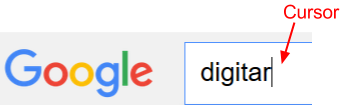
\includegraphics[scale=0.7]{Figures/cursor2}
		\label{fig:cursor2}
		\caption{Cursor se movimentou depois de ter recebido uma palavra}
\end{figure}


\subsubsection{Teclas}

Cada pedacinho do teclado é chamado de \textbf{tecla}, e elas são classificadas em quatro diferentes grupos:

\begin{figure}[!h]
        \centering
		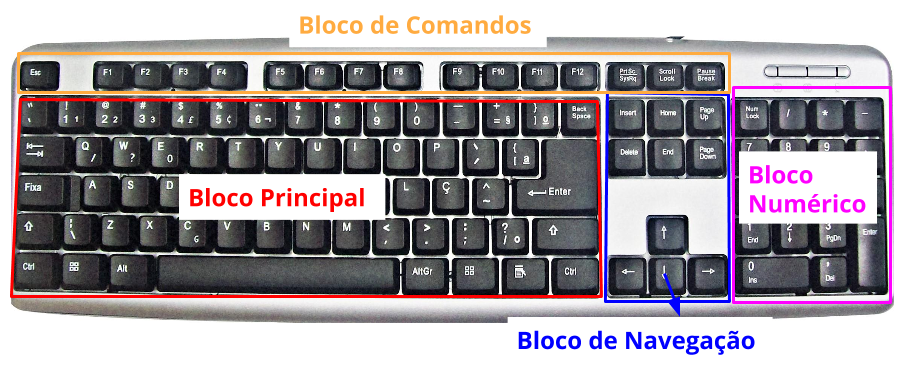
\includegraphics[scale=0.6]{Figures/teclado-blocos}
		\label{fig:teclado-blocos}
		\caption{Blocos/Grupos de teclas com utilidades parecidas}
\end{figure}



\begin{itemize}
	
		\item \textbf{Bloco Principal}: parte do teclado essencial para realmente formular palavras e frases. Aqui estão teclas de letras, pontuação e de caracteres especiais(cifrão, porcentagem, espaço, ...).
		
		\item \textbf{Bloco de Navegação}: aqui estão teclas que servem para deslocar/movimentar coisas. Elas são utilizadas principalmente para movimentar a tela (assim como a roda do mouse) e para movimentar o cursor na hora de digitar.
		
		\item \textbf{Bloco Numérico}: contém números e símbolos matemáticos. Podem ser utilizados, por exemplo, com a calculadora.
		
		\item \textbf{Bloco de Funções ou Comandos}: são teclas especiais para mandar o computador fazer algo. Essas teclas dependem muito de o que cada um faz no computador, por isso não entraremos em detalhes.
		
\end{itemize}	


Abaixo está a descrição do uso das teclas mais importantes e básicas do teclado, no entanto, são informações detalhadas e um pouco avançadas; \emph{recomendadas para uma consulta posterior}. Além disso, cada teclado tem um formato e desenho diferente em suas teclas, por isso, as teclas nas imagens podem ser um pouco diferentes das suas.

\begin{itemize}
    
	\item { \textbf{Shift}: em inglês significa ``trocar''. Assim, enquanto essa tecla estiver pressionada, as outras teclas passarão a ter um outro comportamento (mostrado na própria tecla com um desenho menor). As teclas de letras, por exemplo, aparecerão em sua forma maiúscula. Geralmente os teclados possuem duas teclas Shift em posições diferentes para facilitar a vida de quem está digitando. 
	 
	 \begin{figure}[!h]
	    \centering
		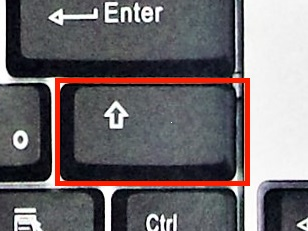
\includegraphics[scale=2]{Figures/shift}
		\label{fig:shift}
		\caption{tecla Shift}
	\end{figure}
	}
	
	\item{ \textbf{Caps Lock}: em inglês significa ``travar maiúsculas''. Quando essa for \emph{ativada}, todas as letras digitadas aparecerão no computador em sua forma maiúscula. A maioria dos teclados possuem um sinal luminoso que permite saber se essa tecla está ativada ou não.
	
    \begin{figure}[!h]
	    \centering
		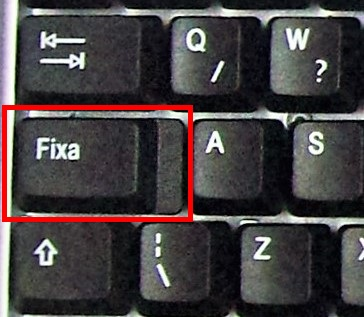
\includegraphics[scale=2]{Figures/caps-lock}
		\label{fig:caps-lock}
		\caption{tecla Caps Lock}
	\end{figure}
    }
    
    \item { \textbf{Num Lock}: em inglês significa ``travar número'' e tem um funcionamento parecido com a tecla Caps Lock. Quando essa tecla estiver \emph{ativada}, as teclas do bloco de números poderam ser utilizadas. Quando desativada, as teclas do bloco de números não funcionarão. A maioria dos teclados possuem um sinal luminoso que permite saber se essa tecla está ativada ou não.

    \begin{figure}[!h]
	    \centering
		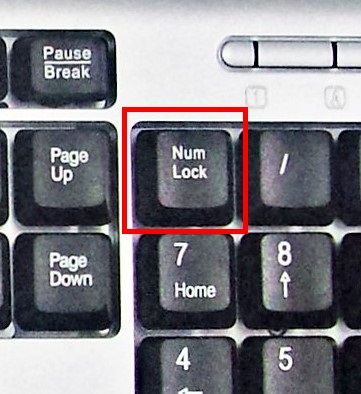
\includegraphics[scale=2]{Figures/num-lock}
		\label{fig:num-lock}
		\caption{tecla Num Lock}
	\end{figure}
	}
	
	\item { \textbf{Enter}: em inglês significa ``confirmar''. Quando você estiver digitando um texto e quiser ``pular'' uma linha, utilize a tecla Enter. Além disso, ela também é bastante utilizada na internet para \textbf{confirmar uma ação}. Geralmente os teclados possuem duas teclas Enter em posições diferentes para facilitar a vida de quem está digitando.
	
	\begin{figure}[!h]
	    \centering
		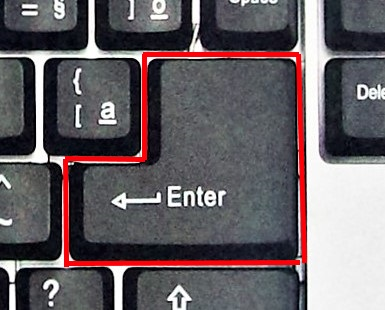
\includegraphics[scale=2]{Figures/enter}
		\label{fig:enter}
		\caption{tecla Enter}
	\end{figure}
	}

	\item { \textbf{Backspace}: em inglês significa ``espaço para trás''. Com essa tecla você consegue \emph{mover o cursor para trás}, \emph{apagando} o que estava naquele lugar.
	
    \begin{figure}[!h]
	    \centering
		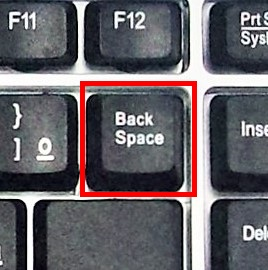
\includegraphics[scale=2]{Figures/backspace}
		\label{fig:backspace}
		\caption{tecla Backspace}
	\end{figure}
	}

	\item { \textbf{Space}: em inglês significa ``espaço''. Ela é a maior tecla do teclado, e tem funcionamento semelhante à Backspace. Quando utilizada, a tecla colocará um espaço em branco onde o cursor estiver, fazendo com que o cursor avance.
    
    \begin{figure}[!h]
	    \centering
		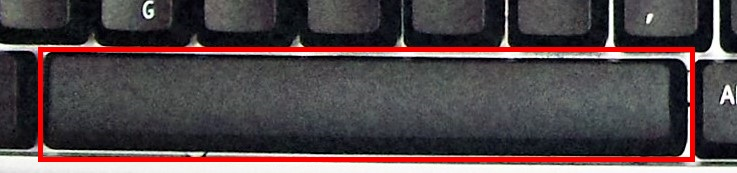
\includegraphics[scale=2]{Figures/space}
		\label{fig:space}
		\caption{tecla Space}
	\end{figure}
	}

	\item { \textbf{Esc}: em inglês significa ``escapar''. Como o nome sugere, ela serve para fechar coisas ou parar de fazer algo.
	
	\begin{figure}[!h]
	    \centering
		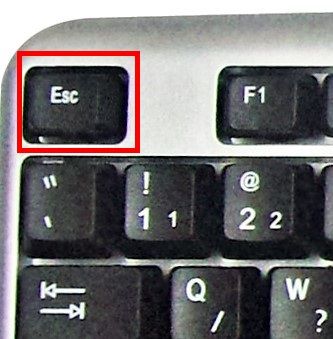
\includegraphics[scale=2]{Figures/esc}
		\label{fig:esc}
		\caption{tecla Esc}
	\end{figure}
	}

\end{itemize}

\subsubsection{Digitação}

Quando se começa a aprender a digitar, é muito comum ficar decepcionado com a velocidade que você digita. Mas saiba que é necessário  prática e dedicação para aprender a digitar de forma fluída e rápida. Assim, há algumas ferramentas digitais que auxiliam nesse treinamento; veremos mais à frente como acessar essas ferramentas pelo seu computador (necessário internet).

Pode parecer estranho, mas digitar com um teclado deu tão certo que pessoas com uma boa digitação conseguem escrever bem mais rápido do que pessoas escrevendo textos com caneta. Além disso, como veremos em um outro capítulo, é muito mais fácil mudar partes do texto quando você estiver utilizando o computador.

\subsection{Monitor}

\begin{figure}[!h]
        \centering
		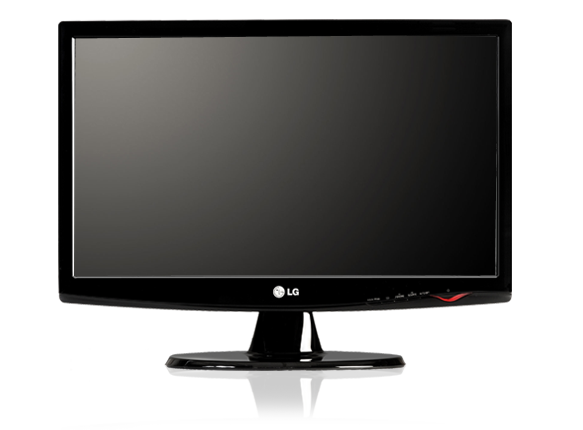
\includegraphics[scale=0.4]{Figures/monitor}
		\label{fig:monitor}
		\caption{Exemplo de um Monitor}
\end{figure}

O monitor é semelhante a uma televisão, só que ele exibe as coisas que estão acontecendo dentro do computador. É por meio do monitor que você consegue ver onde está o ponteiro do Mouse e se as palavras que estão sendo digitadas pelo teclado estão realmente sendo entendidas pelo computador.

Todo monitor, assim como as televisões, possuem um botão de ``Ligar/Desligar'', chamado também de botão ``Power'' (\icon{Figures/power}). Quando você ligar o seu computador, pode ser que o monitor esteja desligado e não apareça nada na tela, por isso, é importante certificar se o botão de ``Ligar/Desligar'' está devidamente ativado.


\section{O Windows 7}

\begin{figure}[!h]
	\centering
	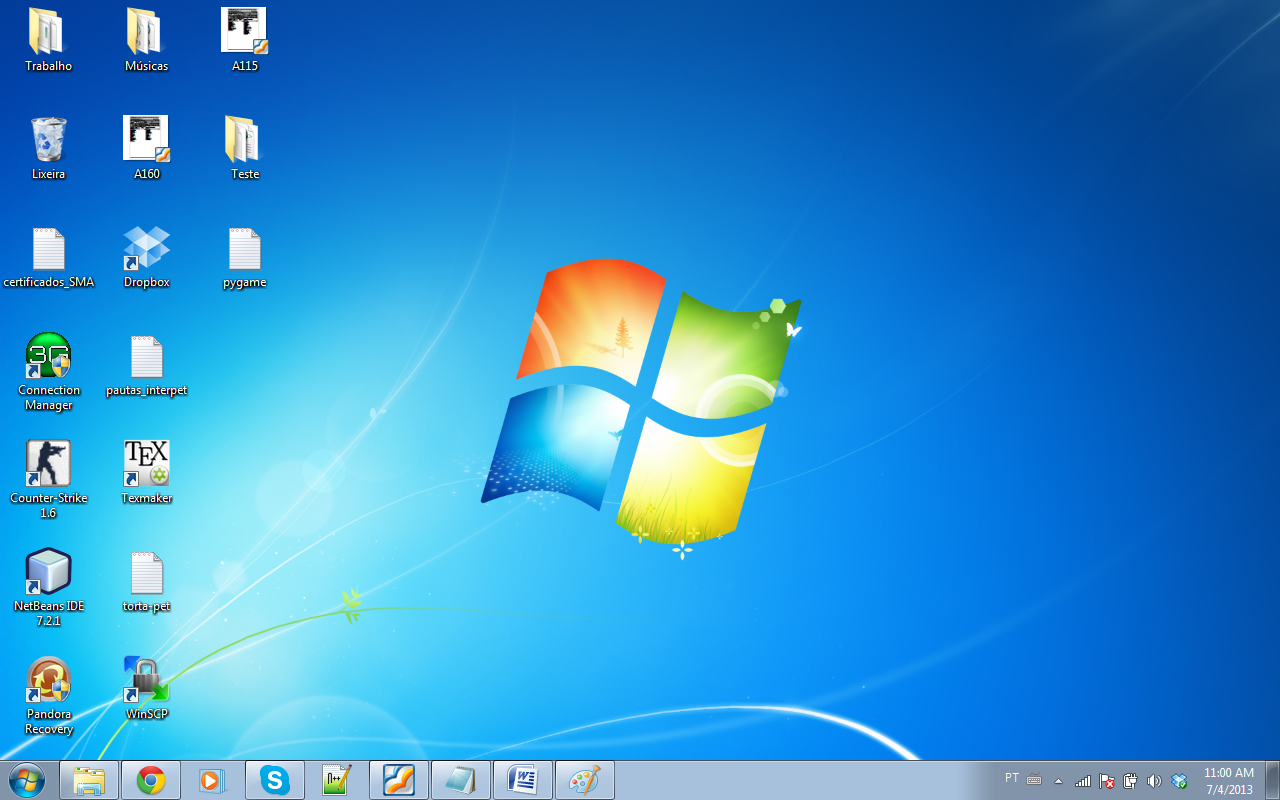
\includegraphics[scale=0.3]{Figures/desktop}
	\caption{Um exemplo do que você pode ver na tela de um computador}
	\label{fig:desktop}
\end{figure}

Todo computador possui uma forma de mostrar ao usuário – pela tela – o que está acontecendo dentro dele. Essa forma dele se mostrar – e de se comportar – é chamada de \textbf{sistema operacional}. O sistema operacional é como se fosse a marca, ou modelo, do computador. Assim, diferentes computadores podem ter sistemas operacionais diferentes.

Nesse curso, utilizaremos o sistema operacional mais comum nos computadores de hoje em dia: o \textbf{Windows 7}. Windows é o nome principal do sistema, e o ``7'' descreve a sua \textit{versão}. No momento em que essa apostila foi feita, já existiam duas versões mais recentes de Windows: Windows 8 e Windows 10. Se o computador da sua casa tiver uma versão mais recente do que a desse curso, não se preocupe. As noções básicas que daremos aqui não mudam de versão para versão; a única coisa que pode mudar é a \textit{aparência} das coisas e os \textit{lugares} em que elas poderão ser encontradas. Assim, pode ser que algumas imagens contidas nessa apostila não reflitam exatamente o que vocês estão vendo em seus computadores. 

No entanto, se o sistema operacional do seu computador for algo muito diferente do Windows, como por exemplo: Ubuntu, MacOS, ou algum outro, pode ficar difícil acompanhar o conteúdo dessa apostila. Nessas condições, recomenda-se pedir ajuda a alguma pessoa experiente e pedir que se instale o Windows - de preferência o 7 - no seu computador.

Nas seções seguintes, começaremos a nos familiarizar com o sistema operacional do nosso computador. Entenderemos melhor o que são essas coisas mostradas na tela do monitor (\textit{interface gráfica}), e aprenderemos como manuseá-las para realizar as tarefas que desejamos.

\subsection{Área de Trabalho (Desktop)}

\begin{figure}[!h]
	\centering
	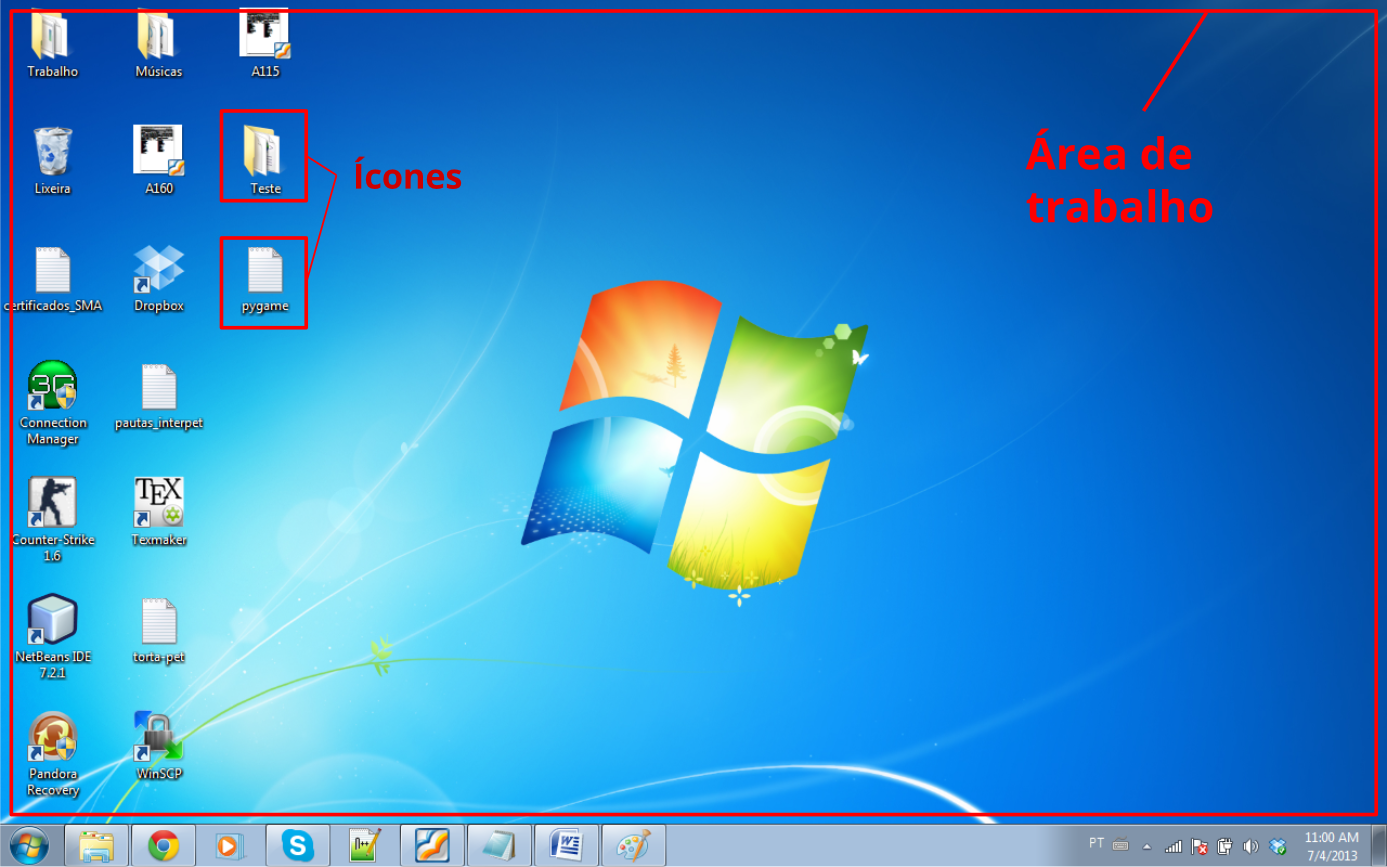
\includegraphics[scale=0.7]{Figures/desktop-notes}
	\caption{Área de trabalho com vários ícones}
	\label{fig:desktop-notes}
\end{figure}

Toda vez que você liga o computador, a primeira coisa que aparece – depois dele ter realmente acabado de se inicializar – é a \textbf{Área de Trabalho}, ou em inglês \textbf{Desktop}. Como o nome sugere, a área de trabalho é um \textit{ambiente virtual} dentro do computador no qual se encontram ferramentas frequentemente utilizadas pelo usuário. 

Certamente, a área de trabalho do seu computador não estará igual à da imagem. Isso acontece porque a área de trabalho é algo customizável, ou seja, você pode – assim como em sua área de trabalho do mundo real – posicionar as ferramentas que você mais utiliza da forma que quiser e mudar a aparência desse ambiente.

\subsubsection{Ícones}

\begin{figure}[!h]
	\centering
	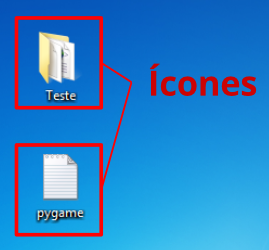
\includegraphics[scale=0.3]{Figures/icones}
	\caption{Dois exemplos de ícones}
	\label{fig:icones}
\end{figure}

Na figura de exemplo, podemos ver que há várias pequenas imagens com um nome embaixo espalhadas pela área de trabalho. Damos o nome de \textbf{ícones} a essas pequenas imagens. Os ícones na área de trabalho servem de atalhos para os programas mais utilizados.

Uma característica importante desses ícones é que eles são \textbf{clicáveis}. Você pode clicá-los de acordo com as maneiras descritas na seção \ref{botoes-mouse} sobre os botões do mouse. 

Você pode também organizar os ícones da área de trabalho: clique com o botão direito do mouse em uma parte vazia do Desktop (para mostrar as ações opcionais), e selecione a opção:

Classificar por $->$ Nome

 \hspace{3.6cm}Tamanho

 \hspace{3.6cm}Tipo de item

 \hspace{3.6cm}Data de modificação.\\

 Existe uma outra opção chamada Exibir. Clicando nela com o botão esquerdo do mouse você pode Organizar ícones automaticamente. Uma outra opção é soltar o ícone em qualquer parte da área de trabalho.


\begin{figure}[!htbp]
	\centering
	\begin{minipage}[b]{0.45\textwidth}
		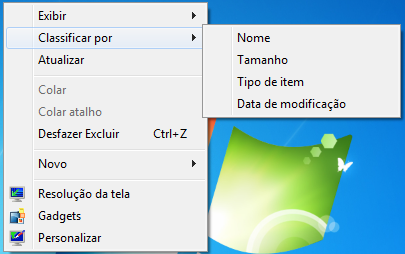
\includegraphics[width=\textwidth]{Figures/icone1}
		\caption{Classificar por}
		\label{fig:classificar por}
	\end{minipage}
	\hfill
	\begin{minipage}[b]{0.53\textwidth}
		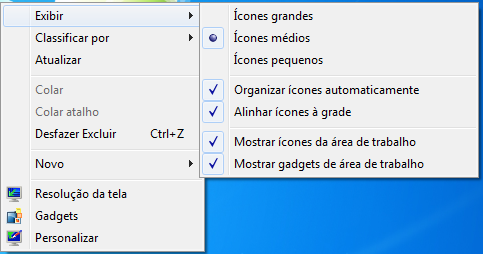
\includegraphics[width=\textwidth]{Figures/icone2}
		\caption{Exibir}
		\label{fig:exibir}
	\end{minipage}
\end{figure}

\subsection{Barra de Tarefas}

É uma barra de ferramentas gráficas usada para controlar a execução dos programas dispostos em janelas, classificando-as como ativa ou inativa. Tem como principal componente o botão iniciar.

É subdividida em:

\begin{itemize}
	\item \textbf{Menu Iniciar} : nele estão organizados todos os programas do computador para um acesso imediato;

	\item \textbf{Barra de Inicialização Rápida} : podem ser colocados nesta área os programas mais utilizados pelo usuário;

	\item \textbf{Janela Ativa ou Inativa} : nesta área aparecem todas as janelas que estão ativas ou inativas (os programas que estão em execução são mostrados);

	\item \textbf{Área de Notificação} os programas que estão sendo controlados pelo sistema aparecem nesta área, inclusive o relógio.

\end{itemize}

\begin{figure}[!h]
	\centering
	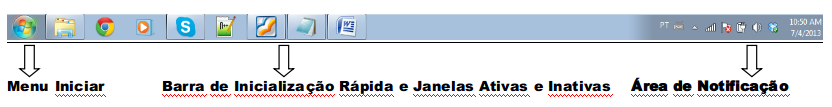
\includegraphics[scale=0.5]{Figures/menu_windows}
	\label{fig:menu_windows}
\end{figure}

\subsubsection{Relógio/Calendário}

O relógio está localizado na direita inferior da barra de tarefas. Para fazer a visualização da data, basta clicar em cima da hora. Para fazer correção de hora e/ou data, basta clicar em {\bf Alterar configurações de data e hora}.

\begin{figure}[!h]
	\centering
	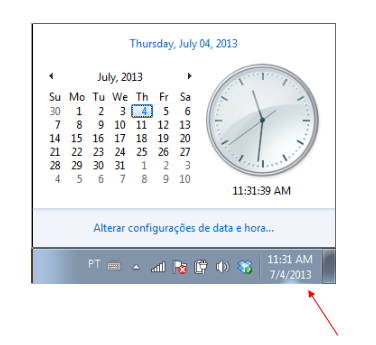
\includegraphics[scale=0.6]{Figures/relogio}
	\caption{Relógio do Windows 7}
	\label{fig:relogio}
\end{figure}

Após serem feitas as modificações de data e hora deve-se clicar no botão {\bf OK} para que as atualizações sejam salvas

\begin{figure}[!h]
	\centering
	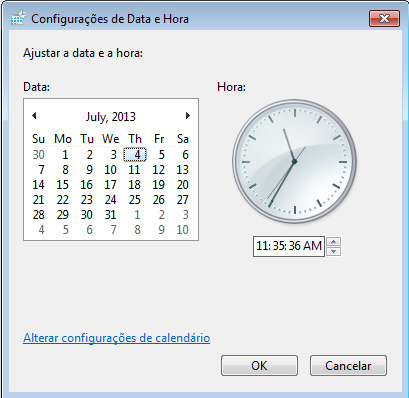
\includegraphics[scale=0.6]{Figures/relogio2}
	\caption{Calendário do Windows 7}
	\label{fig:calendario}
\end{figure}

\subsubsection{Extra}
\begin{enumerate}
	\item Vamos através do calendário descobrir o dia da semana que você nasceu.
\end{enumerate}


\subsubsection{Menu Iniciar}

Por meio do \textbf{Menu Iniciar} podemos acessar os diversos recursos disponíveis em nosso computador. Nele estão contidos todos os programas instalados, diversas ferramentas de manutenção do sistema e ferramentas úteis como a calculadora, bloco de notas e o Google Chrome \footnote{O naveggador padrão é o Internet Explorer, no entanto, o Chrome apresenta melhor desempenho.} que é o programa de navegação na internet . Ao se clicar neste, abrirá no computador uma janela semelhante a da figura abaixo:

\begin{figure}[!h]
	\centering
	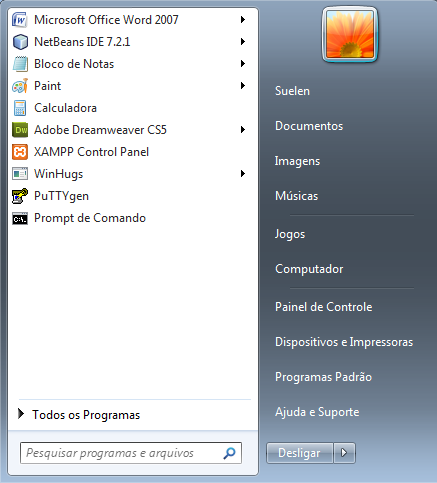
\includegraphics[scale=0.7]{Figures/iniciar}
	\caption{Menu Iniciar}
	\label{fig:iniciar}
\end{figure}

Na coluna da esquerda, fica a lista dos programas usados mais recentemente.

\begin{itemize}
	\item \textbf{Todos os programas} : Nele você encontra os ícones de todos os programas instalados assim como as ferramentas de administração do sistema;

	\item \textbf{Documentos} : Aqui podem ser guardados todos os documentos produzidos no computador;

	\item \textbf{Imagens} : É uma pasta para armazenagem de imagens;

	\item \textbf{Músicas} : É uma pasta que contém ou podem ser armazenados diversos formatos de áudio;

	\item \textbf{Jogos} : Aqui encontra-se todos os jogos disponíveis do computador;

	\item \textbf{Computador} : Aqui você pode ter acesso às pastas do sistema operacional;

	\item \textbf{Painel de Controle} : Contém opções de configuração do computador;

	\item \textbf{Dispositivos e Impressoras} : Aqui se encontram as impressoras e aparelhos de fax instalados no computador;

	\item \textbf{Programas Padrão} : Aqui pode-se definir os programas que o Windows usa por padrão;

	\item \textbf{Ajuda e suporte} : Tire suas dúvidas e encontre soluções para diversos problemas que possam aparecer no sistema operacional;

	\item \textbf{Pesquisar Programas e Arquivos} : Localizar imagens, pastas e arquivos;

	\item \textbf{Desligar} $\rightarrow$ Opções: Trocar usuário, Fazer logoff, Bloquear, Reiniciar, Suspender e Hibernar.
\end{itemize}

\subsection{Janelas}
Existem algumas ferramentas que facilitam a manipulação das janelas que são abertas no ambiente Windows.

\subsubsection{Barra de Rolagem}
Esta barra serve para mover ambientes gráficos dentro das janelas. Podem estar na posição vertical ou horizontal.

\subsubsection{Redimensionando uma janela}
Para redimensionar uma janela, leve o ponteiro do mouse até a quina da janela e arraste até o tamanho desejado.

\begin{figure}[!h]
	\centering
	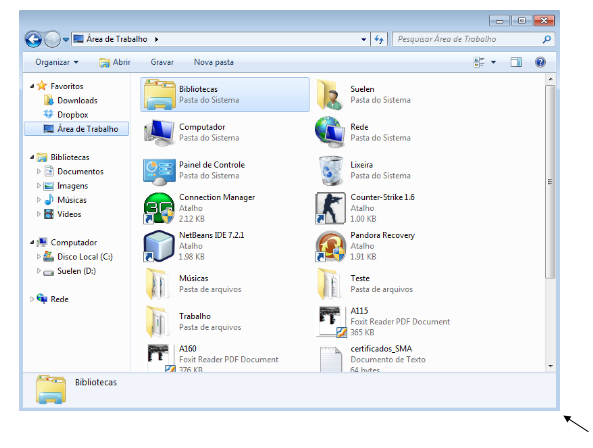
\includegraphics[scale=0.5]{Figures/red_janela}
	\caption{Leve o ponteiro do mouse até a área apontada pela seta como ilustrado acima}
	\label{fig:redimensionando janela}
\end{figure}


\subsubsection{Botões}

\noindent \icon{Figures/minimizar}{\bf Botão Minimizar}: reduz ou minimiza uma janela a um botão da barra de tarefas do Windows (seu programa se torna um ícone da barra de tarefas).

\noindent\icon{Figures/maximizar}{\bf Botão Maximizar}: aumenta ou maximiza uma janela (deixa a janela do tamanho da tela do computador).

\noindent\icon{Figures/restaurar}{\bf Botão Restaurar}: restaura uma janela para o seu tamanho ou posição anterior.

\noindent\icon{Figures/fechar}{\bf Botão Fechar}: fecha um programa ou janela ativa. Caso um arquivo aberto não tenha sido salvo ou contenha alterações não salvas, você será solicitado a salvar ou não o arquivo antes de fechá-lo.

\subsubsection{Movendo uma Janela}

Para mover uma janela, leve o ponteiro do mouse até a barra de títulos. Segure o botão esquerdo do mouse e arraste a janela até a posição desejada.

\begin{figure}[!h]
	\centering
	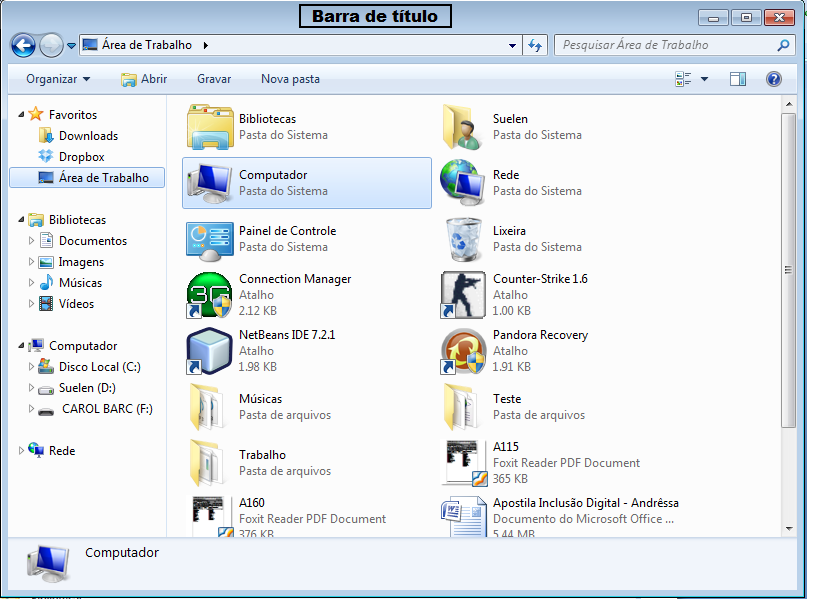
\includegraphics[scale=0.5]{Figures/mov_janela}
	\caption{Ilustração da localização da barra de título}
	\label{fig:movendo janela}
\end{figure}

\subsection{Aplicativos Diversos}

Os programas de computador utilizados diretamente por pessoas comuns, como os editores de texto, são chamados de aplicativos.

O Windows 7 vem com diversos aplicativos nativos e você pode instalar outros de acordo com suas necessidades. Para acessá-los vá até o {\bf Iniciar$>$Todos os programas} e escolher o aplicativo desejado. Alguns aplicativos úteis são:

\begin{itemize}
	\item{
		{\bf Internet Explorer}: Usado para exibir páginas na Internet.
	\vspace{-1.2cm}{
	\begin{figure}[!h]
		
\includegraphics[scale=0.1]{Figures/ie}
		\label{fig:internet explorer}
	\end{figure}}
    }



    \item{
    	{\bf Google Chrome}: Usado para exibir páginas na Internet.
    	\vspace{-1.2cm}{
    		\begin{figure}[!h]
    			
\includegraphics[scale=0.1]{Figures/chrome}
    			\label{fig:chrome}
    		\end{figure}}
    	}

	\item{
		{\bf Mozilla Firefox}: Usado para exibir páginas na Internet.
		\vspace{-1.2cm}{
			\begin{figure}[!h]
				
\includegraphics[scale=0.1]{Figures/firefox}
				\label{fig:firefox}
			\end{figure}}
		}


	\item{
		{\bf Windows Media Player}:reproduzir mídia digital, inclusive músicas, vídeos, CDs e DVDs.
		\vspace{-1.3cm}{
			\begin{figure}[!h]
				
\includegraphics[scale=1.2]{Figures/wmp}
				\label{fig:wmp}
			\end{figure}}
		}

\end{itemize}

Existem em outros diretórios, dezenas de aplicativos para diversas finalidades: Controle de sistemas, redes, teclado virtual, entre outros. Falaremos, mais adiante, de alguns dos principais aplicativos que o Windows disponibiliza.

\begin{itemize}
	\item{
		{\icon{Figures/bloco_notas}\bf Bloco de Notas}: cria e edita arquivos de textos utilizando formatação básica.
		
		}

	\item{
		{\icon{Figures/calculadora}\bf Calculadora}: executa tarefas aritméticas básicas com uma calculadora.
		
		}

	\item{
		{\icon{Figures/paint}\bf Paint}: cria e edita desenhos, além de exibir e editar fotos digitalizadas.
		}
\end{itemize}

\section{Pastas e Arquivos}

É importante mantermos os aplicativos e pastas de trabalho organizados. Em qualquer ambiente de trabalho, organização é fundamental para uma boa produtividade. Também é assim em um sistema operacional. O Windows já vem organizado de forma a facilitar essas rotinas. Contudo, nada impede que organizemos esse ambiente de acordo com nossas necessidades. Não se deve mexer, porém, nas pastas do sistema operacional, sob o risco de danificá-lo.

A organização das pastas e arquivos pode ser observada através do Windows Explorer. Como veremos mais adiante.

\subsection{Criando uma pasta na área de trabalho}

\begin{itemize}
	\item Em uma área vazia do desktop clique no botão direito do mouse. Escolha a opção: {\bf Novo   $\rightarrow $ Pasta};
	\item Nomeie a pasta;
	\item Para abri-la, dê um clique duplo no botão esquerdo do mouse;
	\item Podemos criar uma subpasta dentro da pasta principal utilizando o mesmo processo.
\end{itemize}

	\begin{figure}[!h]
		\centering
		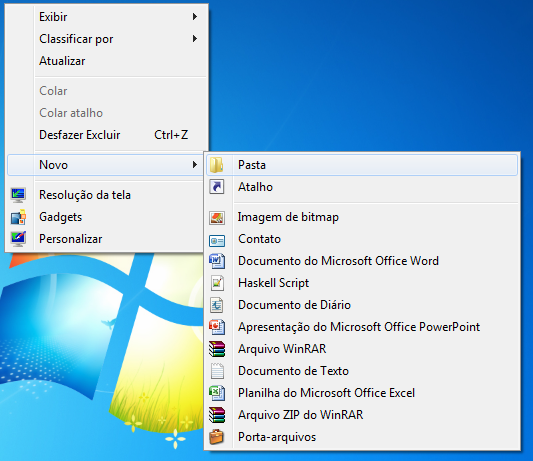
\includegraphics[scale=0.5]{Figures/cria_pasta}
		\caption{Criando pasta}
		\label{fig:criando pasta}
	\end{figure}

\subsection{Windows Explorer}

O Windows Explorer é uma ferramenta que auxilia na organização dos arquivos e pastas do disco rígido (HD).


Para acioná-lo, desça com a seta até o {\bf Menu iniciar $\rightarrow$ Todos os programas $\rightarrow$ Acessórios $\rightarrow$ Windows Explorer}.


\begin{figure}[!h]
	\centering
	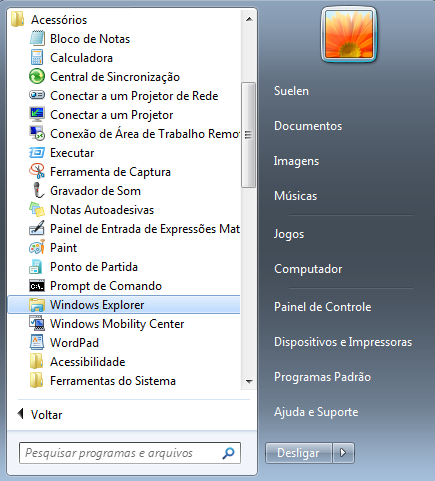
\includegraphics[scale=0.5]{Figures/explorer}
	\caption{Sequência para abrir o Windows Explorer}
	\label{fig:explorer}
\end{figure}


\begin{figure}[!h]
	\centering
	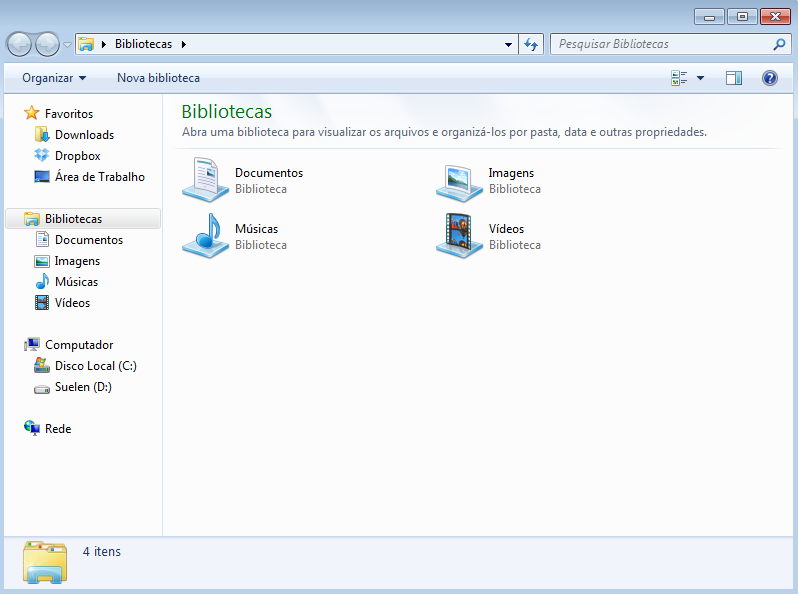
\includegraphics[scale=0.5]{Figures/explorer_pasta}
	\caption{Windows Explorer}
	\label{fig:explorer_p}
\end{figure}

\newpage
\subsection{Criando pastas no Windows Explorer}

\begin{itemize}

	\item Selecionar o ícone {\bf(D:)}: clicando uma vez sobre ele com o botão esquerdo do mouse.
	\item Clique sobre uma área vazia com o botão direito do mouse. Escolha a opção{\bf Novo $\rightarrow$ Pasta}.

	\item Digite o nome da pasta e tecle o botão {\bf Enter}.
\end{itemize}

\begin{figure}[!h]
	\centering
	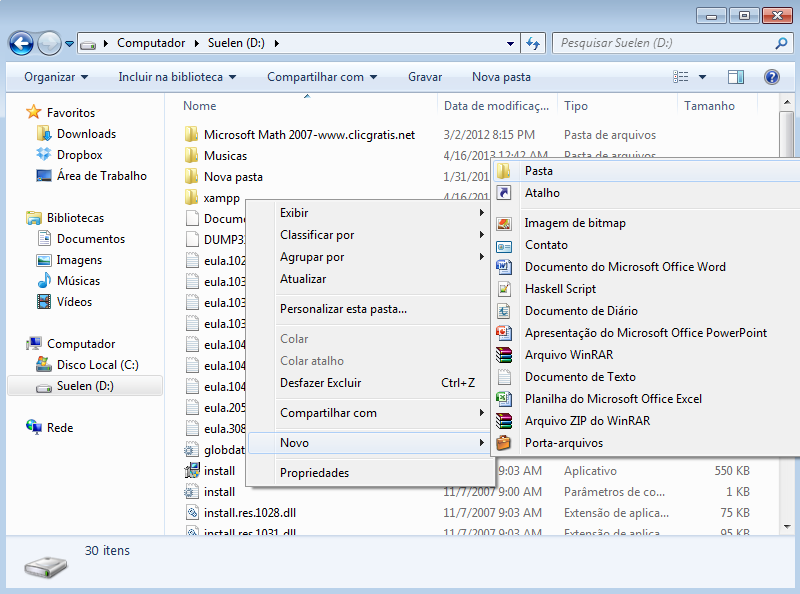
\includegraphics[scale=0.5]{Figures/passo1}
	\caption{Passo 1}
	\label{fig:passo1}
\end{figure}


\begin{figure}[!h]
	\centering
	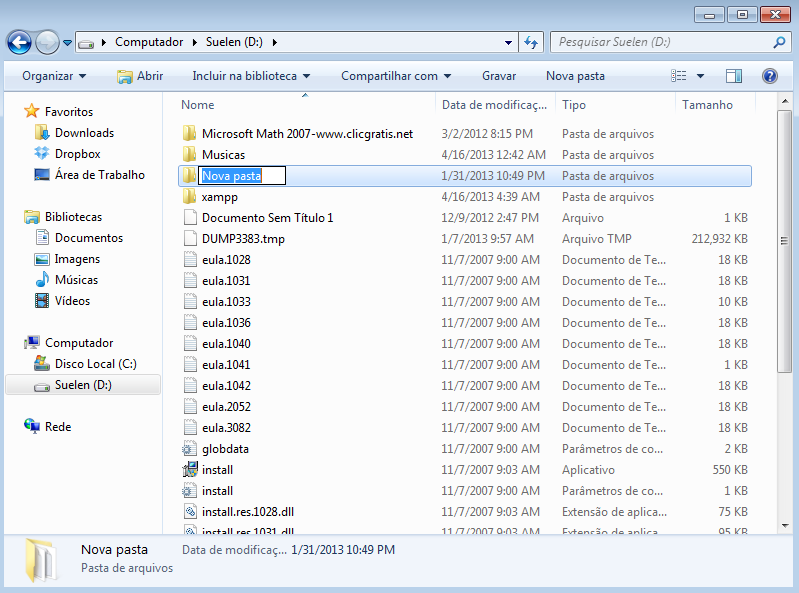
\includegraphics[scale=0.5]{Figures/passo2}
	\caption{Passo 2}
	\label{fig:passo2}
\end{figure}

\subsection{Copiando pastas (ou arquivos)}

\begin{itemize}

	\item Selecionar o item a ser copiado clicando uma vez em cima do ícone com o botão esquerdo do mouse.
	\item Acionar o {\bf Copiar} (ou atalho {\bf Ctrl + C} - você aperta a tecla \textbf{Ctrl} do teclado e enquanto ela está acionada, aperta a letra {\bf C}, soltando ambas ao mesmo tempo).
	\item Selecionar a pasta que irá receber a cópia, clicar com o botão direito em cima do ícone.
	\item E clique na opção {\bf Colar}. Ou então podemos entrar na pasta e utilizar o comando ({\bf Ctrl + V} - você aperta a tecla {\bf Ctrl} do teclado e enquanto ela está acionada, aperta a letra {\bf V}, soltando ambas ao mesmo tempo)
\end{itemize}

\subsection{Movendo Pastas}

\begin{itemize}
	\item Posicionar na pasta que será movida.
	\item Acessar o {\bf Recortar} (atalho {\bf Ctrl + X} - você aperta a tecla Ctrl do teclado e enquanto ela está acionada, aperta a letra {\bf X}, soltando ambas ao mesmo tempo).
	\item Selecionar o local de destino.
	\item Acessar o {\bf Colar}. Ou entrar na pasta e utilizar o atalho ({\bf Ctrl + V}).
\end{itemize}

\subsection{Renomeando Pastas}

\begin{itemize}
	\item Selecionar a pasta, acessar o {\bf Menu Arquivo}(atalho {\bf Alt + A} - você aperta a tecla {\bf Alt} do teclado e enquanto ela está acionada, aperta a letra {\bf A}, soltando ambas ao mesmo tempo) $\rightarrow$ {\bf Renomear} (atalho F2) e digitar o novo nome.
\end{itemize}

\subsection{Apagando pastas e/ou arquivos}

Basta selecionar a pasta e/ou arquivo, pressionar a tecla {\bf Delete} e confirmar pressionando o botão {\bf Sim}.

	\begin{figure}[!h]
		\centering
		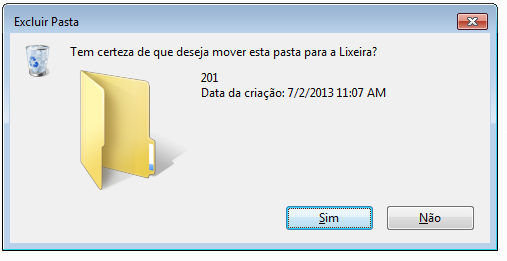
\includegraphics[scale=0.6]{Figures/delete}
		\caption{Janela de Confirmação de Exclusão}
		\label{fig:delete}
	\end{figure}

\subsection{Renomeando Arquivos}

\begin{itemize}
	\item Clicar com o botão direito em cima do ícone a ser renomeado.
	\item Clicar uma vez na opção {\bf Renomear}.
	\item Digitar o novo nome.
	\item Pressionar a tecla {\bf enter}.
\end{itemize}

\subsection{Localizando arquivos e pastas}

\begin{itemize}
	\item Clique uma vez no ícone do Menu {\bf Iniciar}.

	\begin{figure}[!h]
		\centering
		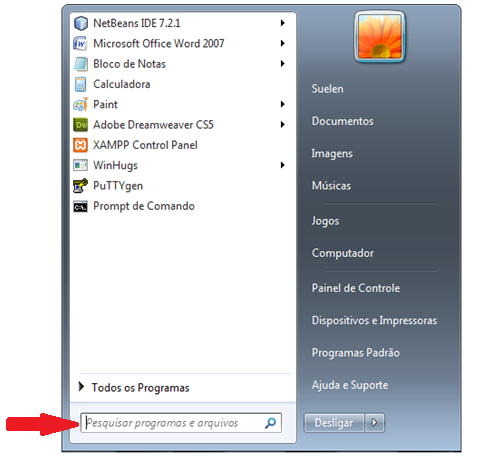
\includegraphics[scale=0.6]{Figures/localizar}
		\caption{Ilustração}
		\label{fig:localizar}
	\end{figure}

	\item  Basta digitar o nome do arquivo, pasta ou programa que deseja pesquisar na área apontada. Depois pressione a tecla {\bf enter}.
\end{itemize}

\subsection{Lixeira}

É acessada através de um ícone na área de trabalho. Nela, são depositados os arquivos excluídos. Enquanto a Lixeira não for limpa, poderemos recuperar os arquivos apagados.

\begin{figure}[!h]
	\centering
	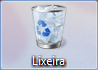
\includegraphics[scale=0.6]{Figures/lixeira}
	\caption{Ícone da lixeira}
	\label{fig:lixeira}
\end{figure}

Para remover definitivamente seu conteúdo, clique no botão do lado direito do mouse e escolha a opção {\bf Esvaziar Lixeira}.

\begin{figure}[!h]
	\centering
	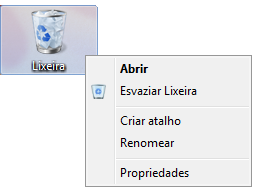
\includegraphics[scale=0.6]{Figures/esvaziar_lixeira}
	\caption{Esvaziar lixeira}
	\label{fig:esvaziar_lixeira}
\end{figure}

Para restaurar um arquivo, acesse a {\bf Lixeira}, escolha o arquivo a ser restaurado, clique nele com o botão direito do mouse, e em seguida clique na opção {\bf Restaurar}.

\begin{figure}[!h]
	\centering
	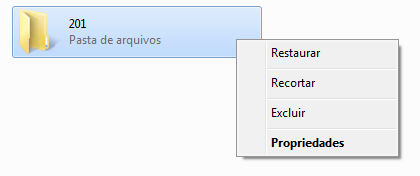
\includegraphics[scale=0.6]{Figures/restaurar_lixeira}
	\caption{Restaurar lixeira}
	\label{fig: restaurar_lixeira}
\end{figure}

\subsection{Exercícios}

\begin{enumerate}
	\item Abra a pasta com o nome de {\bf Fotos} que se encontra na área de trabalho, clicando duas vezes sobre ela com o botão esquerdo do mouse.


	\item Dentro desta pasta estão localizados dois arquivos de imagem com os seguintes nomes: {\bf Árvores} e {\bf Morangos}. Clique duas vezes sobre a imagem com o nome de {\bf Árvores}.

	\item Clique no botão {\bf Maximizar} que se localiza no canto superior direito da janela, do lado esquerdo do botão em vermelho (botão fechar). Note que a janela então expandirá para toda a tela.

	\item Agora clique no botão esquerdo do botão maximizar, o botão {\bf Minimizar}.

	\item Abra a segunda imagem com o nome de {\bf Morangos}. Feche então as duas janelas das imagens abertas.

	\item Agora minimize a janela da pasta {\bf Fotos} e então vá até a área de trabalho e crie uma pasta com o nome de {\bf Minha pasta}.

	\item Vá até a pasta {\bf Fotos} e recorte os dois arquivos de imagens contidos nelas para a pasta {\bf Minha pasta}.

\end{enumerate}

\section{Desenhando com o Paint}

O Paint é um programa que compõe o grupo de acessórios do Windows 7. É um editor de imagens com diversos recursos para executar pequenos trabalhos de edição de imagens. Vamos conhecer as principais funções desse aplicativo e aprender a trabalhar com suas ferramentas.

Na parte superior temos um Menu, uma Barra de ferramentas e uma Paleta de cores. Ao lado da Paleta de cores encontra-se um quadrado que indica a cor ativa no momento. Ao centro se localiza o plano de fundo, onde propriamente trabalhamos com o objeto a ser editado ou criado.

\begin{figure}[!h]
	\centering
	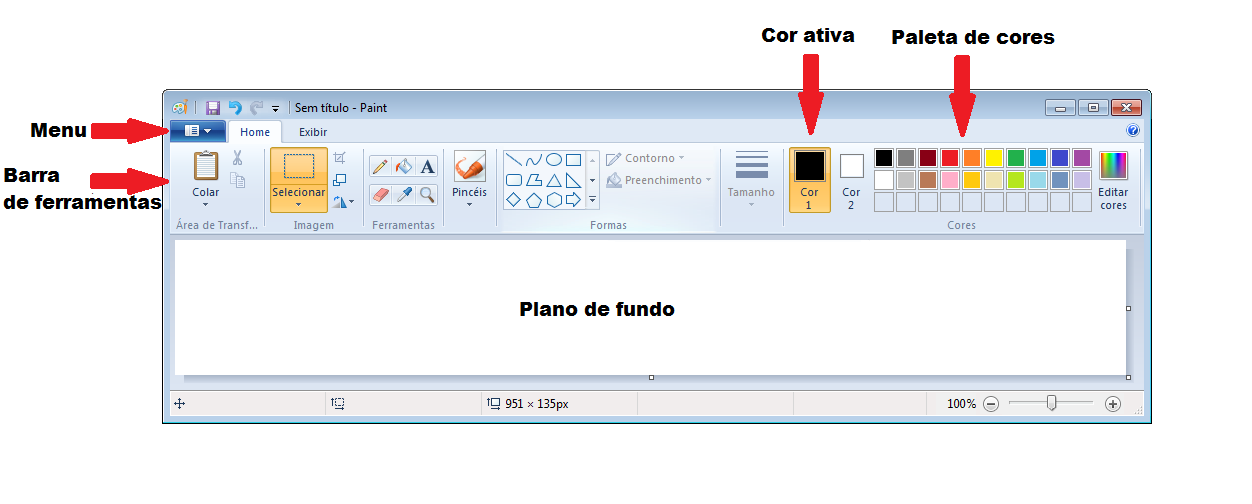
\includegraphics[scale=0.4]{Figures/paint1}
	\label{fig:paint1}
\end{figure}

\subsection{Recursos de desenho}

Os elementos fundamentais de trabalho do Paint residem na sua caixa de ferramentas. O desenho de linhas (retas ou curvas), de figuras prontas (círculo, retângulo, triângulo, etc.), a escrita de texto, o preenchimento de cores, selecionar, apagar, etc., são operações que passam pela ativação de um elemento da caixa de ferramentas.

Por baixo da caixa de ferramentas, existe um retângulo onde é possível visualizar outras opções relacionadas à ferramenta selecionada.


\begin{figure}[!h]
	\centering
	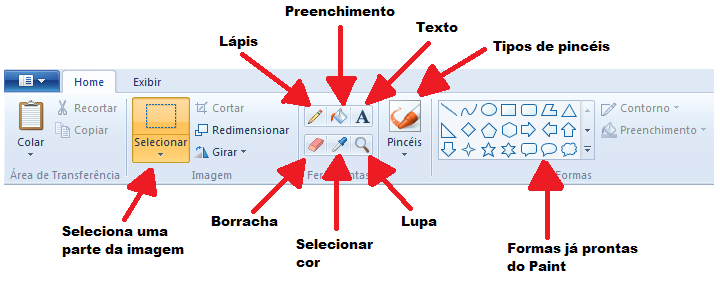
\includegraphics[scale=0.8]{Figures/paint2}
	\label{fig:paint2}
\end{figure}

\subsection{O Menu}

Os arquivos criados pelo Paint por padrão são salvos como bitmap (.bmp). Porém podem ser salvos também em JPEG (.jpg), GIF (.gif), PNG (.png) entre outros.

No Menu, encontre o seguinte ícone:

\begin{figure}[!h]
	\centering
	
\includegraphics[scale=0.8]{Figures/iconep}
	\label{fig:paintp}
\end{figure}

Uma janela abrirá com as seguintes opções:

\begin{itemize}
	\item {\bf Nova} – permite criar um novo arquivo;

	\item {\bf Abrir} – permite abrir um arquivo existente;

	\item {\bf Salvar} – permite gravar o arquivo aberto;

	\item {\bf Salvar como} – permite gravar o arquivo aberto com outro nome, formato ou em outro local;

	\item {\bf Imprimir} – Imprime o arquivo que está sendo editado pelo Paint;

	\item {\bf Definir como plano de fundo da área de trabalho} – Define o arquivo que está sendo editado pelo Paint como imagem de fundo da área de trabalho.

	\item {\bf Sair} – permite fechar o aplicativo.
\end{itemize}
\bigskip
\begin{figure}[!h]
	\centering
	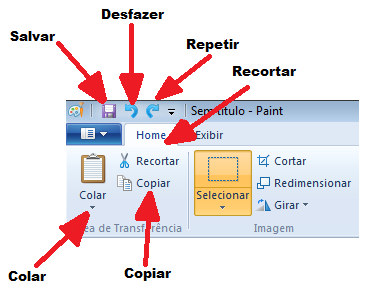
\includegraphics[scale=0.8]{Figures/paint4}
	\label{fig:paint4}
	\caption{Formas de edição no paint}
\end{figure}

\begin{itemize}
	\item {\bf Desfazer} – anula a última ação;

	\item {\bf Repetir} – repete a ação anulada;

	\item {\bf Recortar} – corta a seleção para a Área de Transferência;

	\item {\bf Copiar} – copia a seleção para a Área de Transferência;

	\item {\bf Colar} – insere o conteúdo da Área de Transferência;

	\item {\bf Salvar} – salva o arquivo que está sendo editado.
\end{itemize}

\section{Calculadora}

A calculadora do Windows 7 é acionada através do caminho: {\bf Iniciar $\rightarrow$ Todos os programas $\rightarrow$ Acessórios $\rightarrow$ Calculadora}. Pode ser utilizada através do mouse ou com o uso do teclado numérico.

No item Exibir, você pode alternar a visualização da calculadora entre Padrão e Científica, Programador e Estatística.

\begin{figure}[!h]
	\centering
	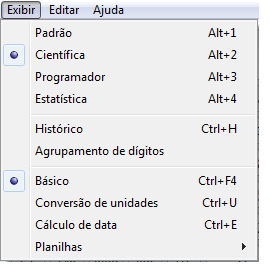
\includegraphics[scale=0.7]{Figures/calc1}
	\label{fig:calc1}
	\caption{Exibir}
\end{figure}

\begin{figure}[!h]
	\centering
	\includegraphics[scale=0.7]{Figures/calc2}
	\label{fig:calc2}
	\caption{Calculadoras Padrão e Científica, respectivamente}
\end{figure}

\subsection{Exercícios}

\begin{enumerate}
\item Abra o aplicativo referente à calculadora ({\bf Iniciar $\rightarrow$ Todos os programas $\rightarrow$ Acessórios $\rightarrow$ Calculadora}). Clique no número 6, multiplique por 64, subtraia 20 e divida por 7.

\item Vamos agora ver quantos dias você possui desde que nasceu, para isso entre em \textbf{Exibir} $\rightarrow$ \textbf{Cálculo de data (Ctrl + E)}, agora na nova aba que se abriu coloque a data inicial, por exemplo, seu aniversário e data de hoje, por fim clique em calcular e voilà.
\end{enumerate}

\section{Microsoft Office 2007}

\subsection{Apresentação}

O Word 2007 faz parte do pacote de produtividade Microsoft® Office System de 2007, que sucedeu ao Office 2003.

Seu principal objetivo é a criação e edição de textos, porém existem ainda várias outras ferramentas muito úteis para o usuário.

\subsection{Executando o Programa}

\begin{itemize}
	\item Dê um clique no botão \textbf {Iniciar};

	\item Posicione a seta do mouse sobre \textbf{Todos os Programas};

	\item Posicione a seta do mouse sobre \textbf{Microsoft Office};

	\item Posicione a seta do mouse e dê um clique sobre \textbf{Microsoft Office Word 2007}.
\end{itemize}

\begin{figure}[!h]
	\centering
	\includegraphics[scale=0.5]{Figures/office1}
	\label{fig:office1}
	\caption{Abrindo o Microsoft Office 2007}
\end{figure}


\subsection{Ambiente de Trabalho}

\begin{figure}[!h]
	\centering
	\includegraphics[scale=0.5]{Figures/office2}
	\label{fig:office2}
	\caption{Conhecendo o Microsoft Office 2007}
\end{figure}


\subsection{Criando Texto}

\begin{itemize}
	\item Clique na área de trabalho;

	\item Digite o texto a seguir:
\end{itemize}


{\textbf{\hspace{5cm} Para refletir}}

``A melhor de todas as coisas é aprender. O dinheiro pode ser perdido ou roubado, a saúde e força podem falhar, mas o que você dedicou à sua mente é seu para sempre.'' (\emph{Louis L'Amour}).


\subsection{Editando Texto}

\begin{itemize}
	\item Selecione o título com o mouse;

	\item Altere as características da fonte como desejar;

	\item Agora vamos alterar as características do texto, basta seguir os passos anteriores;

	\item Não se esqueça de alinhar seu texto da melhor maneira possível.
\end{itemize}


\subsection{Salvando o documento}

\begin{itemize}
	\item Clique no menu \textbf{Office}:

	\begin{figure}[!h]
		\centering
		\includegraphics[scale=0.5]{Figures/office3}
		\label{fig:office3}
		\caption{Salvando um documento}
	\end{figure}

	\item Clique no botão \textbf{Salvar}:

	\begin{figure}[!h]
		\centering
		\includegraphics[scale=0.5]{Figures/office4}
		\label{fig:office4}
	\end{figure}


	\item Encontre o local desejado para guardar seu documento, dê o nome desejado e clique em \textbf{Salvar};

	\item Pronto, agora seu arquivo está guardado em seu computador. Poderá utilizar e alterá-lo sempre que desejar

\end{itemize}

	
\subsection{Criando um novo Documento}

\begin{itemize}

	\item Clique no \textbf{botão Office} e escolha opção \textbf {Novo};

	\item A janela a seguir abrirá:


	\begin{figure}[!h]
		\centering
		\includegraphics[scale=0.47]{Figures/office5}
		\label{fig:office5}
		\caption{Criando um novo documento}
	\end{figure}

	\item Clique em \textbf{Criar};

	\item Novo documento foi aberto e está pronto para ser utilizado;

\end{itemize}


\subsection{Abrindo um documento}

\begin{itemize}
    \item Abra o Word como foi explicado anteriormente;
    
    \item Clique no botão \textbf{Office} e escolha a opção \textbf{Abrir};
    
    \item A seguinte janela abrirá:
    
        \begin{figure}[!h]
        	\centering
        	\includegraphics[scale=0.5]{Figures/office6}
        	\label{fig:office6}
        	\caption{Janela para abrir documentos}
        \end{figure}
    
    \item Procure o local onde se encontra o arquivo desejado. Clique nele e depois em \textbf{Abrir};
    
    \item Para praticar, formate novamente seu texto, alternando fonte, tamanho, cor, dentre outros.
\end{itemize}

\subsection{Desfazendo e Refazendo uma Ação}


\begin{figure}[!h]
	\centering
	\includegraphics[scale=1]{Figures/office7}
	\label{fig:office7}
	\caption{Botões desfazer e refazer}
\end{figure}

\icon{Figures/desfazer} \textbf{Desfazer} - caso você cometa algum erro, ou deseje desfazer uma ação, para voltar ao que era antes, basta clicar no botão desfazer, ele desfaz a última ação que você fez no Microsoft Word. Outra opção para desfazer o que foi digitado é utilizar o atalho do teclado \textbf{Ctrl + Z};\\

\icon{Figures/refazer} \textbf{Refazer} - o botão refazer só é acionado se você utilizar o botão desfazer, o refazer refaz novamente a ação que você desfez através do botão desfazer, seja um erro ou qualquer outra ação.

Para treinarmos a função desses botões siga os passos abaixo:

\begin{enumerate}
	\item Dê um clique no botão \icon{Figures/novo} \textbf{Novo} para abrir um novo documento;

	\item Escolha o tamanho de fonte \textbf{20};

	\item  Digite a palavra: \textbf{Treinamento!}


	\item Selecione a palavra que você acabou de digitar e em seguida pressione a tecla \textbf{Delete};

	\item Dê um clique no botão \icon{Figures/desfazer} Desfazer. Observe que a palavra digitada retornou  a tela.

	\item Agora dê um clique no botão \icon{Figures/refazer} Refazer.
\end{enumerate}

Observe que a palavra digitada foi apagada novamente, pois foi refeita sua última ação, a qual foi apagar a palavra.


\subsection{Recortar, Copiar, Colar}

\icon{Figures/recortar} \textbf{Recortar} - Você pode recortar qualquer coisa que estiver selecionada e depois colá-la em outro lugar. (Quando você recorta algo, você retira de um local e pode colocar em outro). Outra opção para recortar o que foi digitado é utilizar o atalho do teclado \textbf{Ctrl + X};

\icon{Figures/copiar} \textbf{Copiar} - O botão copiar serve para você copiar o que estiver selecionado e depois colá-lo em outro lugar. (Quando você utiliza a opção copiar, você está duplicando o que copiou). Outra opção para copiar o que foi digitado é utilizar o atalho do teclado \textbf{Ctrl + C};

\icon{Figures/colar} \textbf{Colar} - O botão colar só pode ser utilizado depois de você ter \textbf{recortado} ou \textbf{copiado} algo. (O item recortado ou copiado será colado onde o cursor estiver posicionado).

\subsection{Treinamento}

\begin{enumerate}
	\item Escolha o \textbf{Tamanho de Fonte 29};

	\item Digite em letras Maiúsculas: \textbf{TREINAMENTO};

	\item Selecione o que você digitou;

	\item Dê um clique no botão \icon{Figures/copiar} \textbf{Copiar} ou utilize o atalho \textbf{Ctrl + C};

	\item Retire a Seleção clicando em algum lugar da página de texto;

	\item Posicione o cursor no final da linha e pressione \textbf{Enter};

	\item Dê um clique no botão \icon{Figures/colar} \textbf{Colar} ou utilize o atalho \textbf{Ctrl + V};

	\item Dê novamente um clique no botão \icon{Figures/colar}  \textbf{Colar} (Observe que você duplicou a palavra);

	\item Pressione a tecla \textbf{Enter};

	\item Escolha o tamanho de fonte \textbf{35};

	\item Digite em letras maiúsculas: \textbf{TREINAMENTO};

	\item Pressione \textbf{Enter};

	\item Digite em letras maiúsculas: \textbf{INFORMÁTICA};

	\item Pressione \textbf{Enter};

	\item Digite em letras maiúsculas: \textbf{NEP – Laguna};

	\item Pressione \textbf{Enter};

	\item Selecione a linha \textbf{INFORMÁTICA};

	\item Dê um clique no botão  \icon{Figures/recortar} \textbf{Recortar} - ou utilize o atalho \textbf{Ctrl + X};

	\item Posicione o cursor no final da linha \textbf{NEP – Laguna};

	\item Pressione \textbf{Enter};

	\item Dê um clique no botão \icon{Figures/colar} \textbf{Colar} (Observe que as palavras recortadas anteriormente aparecem no local onde você deixou o cursor).

	\item Agora \textbf{Salve} as Alterações em sua pasta com o nome de \textbf{Exercício 04}.
\end{enumerate}

\subsection{Exercícios}

\begin{enumerate}
	\item Para praticar os conhecimentos adquiridos e sua digitação, dê um clique no botão \icon{Figures/novo}
	 \textbf{Novo} para abrir um novo documento;

	\item Digite o seguinte texto para praticar acentuação, não esqueça os marcadores.

	\begin{enumerate}
		\item Palavras com Acento Agudo:
		Pó, Café, Boné, Saúde, Água, Vídeo, Vovó.

		\item Palavras com Acento Circunflexo: Vê, Têm, Silêncio, Eletrônica, Vovô, Crochê, Crê.

		\item Palavras com Cedilha: Laço, Braço, Abraço, Berço, Força, Espaço, Faço.

		\item Palavras com Til: Coração, Emoção, Avião, Tentação, Tubarão, Aplicação
    \end{enumerate}


	\item Altere o texto dando-lhe uma boa aparência. Crie um título.
\end{enumerate}

\subsection{Inserindo uma Imagem no documento}

O Microsoft Word oferece o recurso de se adicionar ao documento imagens que estejam no computador.

\begin{enumerate}
	\item Dê um clique no botão \icon{Figures/novo} \textbf{Novo} para abrir um novo documento;

	\item Dê um clique no \textbf{Menu Inserir}, em seguida no ícone \icon{Figures/imagem};

	\item Observe que abrirá a janela \textbf{Inserir Imagem}. Esta janela será utilizada para encontrar a imagem desejada, que está no computador;

	\item Clique em \icon{Figures/desk} e em seguida selecione a imagem \textbf{Tulipa} e clique em \textbf{Inserir}, ou simplesmente dê um duplo clique na imagem desejada;

	\item Dê UM clique sobre a figura;
	
	\begin{figure}[!h]
		\centering
		\includegraphics[scale=1]{Figures/tulipa}
		\label{fig:tulipa}
		\caption{Figura da Tulipa}
	\end{figure}


	\item Observe que a figura ficou cercada por 8 pontos. Eles servem para \textbf{Aumentar} ou \textbf{Diminuir} a imagem, sempre que você desejar alterar o tamanho posicione a seta sobre um dos 4 cantos de modo que apareça uma seta dupla (você deve alterar o tamanho pelos cantos para que a imagem não fique achatada);

	\item Agora tente alterar o tamanho de sua Imagem. Feito isso clique novamente sobre a mesma e pressione a tecla \textbf{DELETE}.
\end{enumerate}

\subsection{Treinando a Inserção de Imagens}

\begin{enumerate}
	\item Escolha o tamanho de fonte \textbf{14};

	\item Digite o texto abaixo seguindo as formatações e inserindo imagens que você goste e estejam na Área de trabalho (desktop):
\end{enumerate}
		

{\centering \textbf{AMOR}\\

Amor é fogo que arde sem se ver;
\begin{figure}[!h]
	\centering
	\includegraphics[scale=0.3]{Figures/trevo}
\end{figure}

É ferida que dói e não se sente;
\begin{figure}[!h]
	\centering
	\includegraphics[scale=0.3]{Figures/urso}
\end{figure}

É um contentamento descontente;

\begin{figure}[!h]
	\centering
	\includegraphics[scale=0.6]{Figures/coracao}
\end{figure}
É dor que desatina sem doer.

}
\bigskip

3. Agora, \textbf{Salve} em sua pasta com o nome de \textbf{Exercício 07}.

\section{Internet}

\subsection{O que é a Internet}

A Internet permite que uma pessoa em um computador, com acesso a Internet, consiga comunicar (trocar informações) com um outro computador em qualquer lugar do mundo de forma rápida e fácil. Assim, a Internet é uma coleção de computadores que estão conectados entre si.

Ela surgiu de um projeto militar do governo americano no início da década de 50, mas se expandiu e já conta com aproximadamente 2 bilhões de usuários, sendo, pelo menos, 100 milhões de brasileiros. Atualmente, ela é parte indispensável da vida de boa parte das pessoas.


\subsection{Conceitos Básicos da Internet}


\subsubsection{Site}

É uma coleção de páginas web, isto é, de documentos acessíveis através da web, na internet. Os sites da Internet, em geral, podem ter os seguintes propósitos:

\textbf{Institucional}: muitas empresas usam seus sites como ponto de contato entre uma instituição e seus clientes ou fornecedores. Instituições comerciais podem usar seus websites para comércio eletrônico ou até para recrutamento.

Ex.: http://www.ufu.br/ (Site da Faculdade de Engenharia Mecânica da UFU);\\


\textbf{Informações}: veículos de comunicação como jornais, revistas, agências de notícias ou mesmos jornalistas independentes utilizam a Internet para veicular notícias, por meio de seus sites.

Ex.: \url{http://www.joelmirbeting.com.br}/(blog do jornalista especialista em economia Joelmir Beting);\\


\textbf{Aplicações}: existem sites cujo conteúdo contém processadores de texto, planilhas eletrônicas, editores de imagem, softwares de correio eletrônico, agendas, etc.

Ex.: \url{http://docs.google.com} (exemplo de site que apresenta as ferramentas do desktop);\\


\textbf{Comunitário}: são os sites que servem para a comunicação de usuários com outros usuários da rede. Nesta categoria se encontram os chats, fóruns e sites de relacionamento.

Ex.: \url{http://www.facebook.com/};\\


\textbf{Portais}: são chamados de ``portais'' os sites que congregam conteúdos de diversos tipos entre os demais tipos, geralmente fornecidos por uma mesma empresa. Recebem esse nome por congregarem a grande maioria dos serviços da Internet num mesmo local.

Ex.: \url{http://g1.globo.com/}.\\


\subsubsection{Domínio}

Todo site tem no final de seu endereço uma palavra que definimos como domínio. O domínio serve, para identificar a natureza dos sites. Por exemplo, o site do Banco do Brasil http://www.bb.com.br tem o domínio COM. Já o site http://www.sosmatatlantica.org.br tem o domínio ORG. Os principais domínios são: \textbf{.com / .gov / .edu / .mil / .org}\\

\textbf{URL ou Endereço Eletrônico}

\begin{figure}[!h]
	\centering
	\includegraphics[scale=0.5]{Figures/site}
	\label{fig:site}
	\caption{Representação de um site}
\end{figure}

\begin{enumerate}
	\item A expressão WWW representa a expressão do inglês world wide web que em português quer dizer rede mundial de computadores;

	\item Nome do site;

	\item Domínio;

	\item Localização do site. O BR significa que o site é brasileiro.
\end{enumerate}


\subsubsection{Links}
Texto colorido e sublinhado ou uma figura em que o internauta clica para ir à uma página da internet. O usuário nunca deve acessar links que não conheça, uma vez que, estes links podem instalar programas maliciosos no computador.

Se você estiver acessando a apostila pelo computador, clique neste texto(ele é um link que te levará para um site).\\
\textbf{Link}: \url{www.google.com.br}


\subsubsection{Browser ou Navegador}

Programa que permite aos usuários da internet consultar páginas e navegar. Existem vários navegadores no mercado, dentre eles podemos citar:

\begin{itemize}
	\item \textbf{Internet Explorer} : Desenvolvido pela Microsoft. Sua última versão apresentou vários problemas de segurança, por isso recomenda-se a utilização do Firefox ou do Chrome;
	\item \textbf{Microsoft Edge} : Também desenvolvido pela Microsoft, seu uso é similar ao do Explorer. Esse navegador ja vem instalado em sistemas mais recentes da Microsoft;
	\item \textbf{Mozilla Firefox} : Seu uso é similar ao do Explorer;
	\item \textbf{Opera} : Seu uso é similar ao do Explorer;
	\item \textbf{Google Chrome} : navegador desenvolvido pela Google. É o mais seguro e eficiente.
\end{itemize}

\textbf{OBS}.: Não se recomenda o uso do Internet Explorer.

\section{Conhecendo o Google Chrome}
		
\subsection{Tela Principal}
A tela principal do Google Chrome pode ser divida basicamente em três partes: área de digitar o site, área de exibição do conteúdo e área de indicadores.

\subsection{Menus}

\begin{enumerate}
	\item \textbf{Abrindo uma nova guia} : Ter várias guias significa ter vários sites abertos ao mesmo tempo. Abrir uma nova guia é simples ! Você pode apertar \textbf{Ctrl+T} ou clicar no botão do lado da primeira guia e assim por diante.
	
    	\begin{figure}[!h]
    		\centering
    		\includegraphics[scale=0.45]{Figures/gc8}
    		\label{fig:googlechromeguia}
    	\end{figure}
		
	\item \textbf{Favoritos} : Ás vezes, nós desejamos “guardar” o endereço de um site para o acessarmos mais tarde. Para isso, os navegadores dispõe da ferramenta “Favoritos”.
	
	Para fazer com que a barra de favoritos fique sempre visível, bas ir em \icon{Figures/gc1}  $\rightarrow$ \textbf{Configurações} e, na seção de \textbf{Aparência}, marcar a opção \textbf{Sempre mostrar a barra de favoritos}
	
	\begin{figure}[!h]
		\centering
		\includegraphics[scale=0.65]{Figures/gc2}
		\label{fig:googlechrome}
	\end{figure}
	
	Finalmente, para adicionar um site aos favoritos deve-se utilizar o atalho \textbf{Ctrl+D} apertar no ícone \icon{Figures/gc5} que fica na barra de endereço. 
	
	\begin{figure}[!h]
		\centering
		\includegraphics[scale=0.45]{Figures/gc7}
		\label{fig:googlechrome7}
	\end{figure}
	Depois disso, aperte o botão \textbf{Concluir} 
	
	Se um site ja estiver favoritado a estrela ficará amarela \icon{Figures/gc6}.
	
	\item \textbf{Imprimir} : Para imprimir no Google Chrome basta ir em \icon{Figures/gc1} $\rightarrow$ \textbf{Imprimir} ou simplesmente apertar \textbf{Ctrl+P}. Uma janela semelhante a essa abrirá.
	
	\begin{figure}[!h]
		\centering
		\includegraphics[scale=0.35]{Figures/gc3}
		\label{fig:gc3}
	\end{figure}
	
	Após isso, basta clicar no botão \textbf{Imprimir}
	
	\newpage
	\item \textbf{Barra de Endereços} : A barra de endereço é o local onde digitamos o site.
	\begin{figure}[!h]
		\centering
		\includegraphics[scale=0.35]{Figures/gc4}
		\label{fig:gc4}
		
	\end{figure}
	
\end{enumerate}

\subsection{Chega de propaganda !}

Muita gente reclama da alta quantidade de janelas que abrem de repente quando estamos mexendo no computador. Esses anúncios quase sempre tem conteúdo indesejado para nós. Uma maneira simples de nos livrarmos disso é instalando um add-on (aplicativo para o navegador) do chrome. Faça o seguinte:

\begin{enumerate}
	\item Pesquise por \textbf{Chrome Web Store} e clique no primeiro link;

	\begin{figure}[!h]
		\centering
		\includegraphics[scale=0.4]{Figures/chrome1}
		\label{fig:chrome1}
		\caption{Pesquisa}
	\end{figure}

	\item No site, pesquise por Adblock e, na parte de extensões, clique em usar no chrome.

	\begin{figure}[!h]
		\centering
		\includegraphics[scale=0.4]{Figures/chrome2}
		\label{fig:chrome2}
		\caption{Pesquisa}
	\end{figure}

\end{enumerate}

Após instalar o Adblock, um ícone, na parte superior direita, será fixado no seu navegador. Veja a diferença do mesmo site com, e sem o Adblock.

\begin{figure}[!htbp]
	\centering
	\begin{minipage}[b]{0.5\textwidth}
		\includegraphics[width=\textwidth]{Figures/adblock1}\\

	\end{minipage}
	\hfill
	\begin{minipage}[b]{0.5\textwidth}
		\includegraphics[width=\textwidth]{Figures/adblock2}

	\end{minipage}
\end{figure}


\subsection{Email no Gmail!}

 O e-mail é um recurso da internet que permite aos usuários receber e enviar mensagens e textos. Por meio dele, mensagens podem ser enviadas para qualquer parte do mundo, possibilitando trocas de informações de forma rápida e extremamente eficiente.

Um e-mail é composto por um Login, o símbolo de arroba (@) e pelo provedor de e-mail. O login é algo que identifica o dono do e-mail. Pode ser um nome de uma pessoa ou um apelido. O provedor do e-mail indica em qual site ele foi cadastrado. Exemplo:\\

\hspace{3.7cm}\textbf{\large{fulano@gmail.com.br}}\\

Nesse caso o login é fulano e o provedor é Gmail.


\subsubsection{Criando uma conta do e-mail no Gmail}

\begin{enumerate}
	\item  Acesse um site de algum provedor de e-mail. No nosso caso abriremos uma conta no Gmail! (\url{www.gmail.com}).
	\item Clique em criar uma conta (na parte superior do site):
    	\begin{figure}[!h]
    		\centering
    		\includegraphics[scale=0.35]{Figures/gmail1}
    		\label{fig:gmail1}
    		\caption{Criando Conta}
    	\end{figure}

    \item  Preencha o formulário de cadastro com seus dados pessoais, login e senha:

        \begin{figure}[!h]
        	\centering
        	\includegraphics[scale=0.2]{Figures/gmail3}
        	\label{fig:gmail3}
        	\caption{Cadastrando}
        \end{figure}

\end{enumerate}

Após entrar no e-mail, você obterá uma página semelhante a essa:

\begin{figure}[!h]
	\centering
	\includegraphics[scale=0.27]{Figures/gmail2}
	\label{fig:gmail2}
	\caption{Gmail}
\end{figure}

Pela figura, podemos observar que a página principal do e-mail possui algumas pastas. Um e-mail geralmente possui 5 pastas principais:

\begin{itemize}
	\item \textbf{Entrada} – e-mails que você recebeu;

	\item \textbf{Rascunho} – mensagens que você escreveu, mas não enviou ainda;

	\item \textbf{Enviadas} – mensagens que você escreveu e enviou;

	\item \textbf{Spam} –é o termo pelo qual é comumente conhecido o envio, a uma grande quantidade de pessoas de uma vez, de mensagens eletrônicas, geralmente com cunho publicitário, mas não exclusivamente;

	\item \textbf{Lixeira} – mensagens que você recebeu e apagou.

	\item \textbf{Botão “1”} – Escrever um novo e-mail

	\item \textbf{Parte “2”} – Caixa de entrada do e-mail, onde fica armazenado suas conversas.

	\item \textbf{Parte “3”} – Bate-papo do gmail, é possivel conversar com seus contatos quando eles estão online

	\item \textbf{Parte “4”} – Opções do seu e-mail.

\end{itemize}


\subsubsection{Lendo e-mails}

Para ver algum e-mail que você tenha recebido, devemos acessar a pasta \textbf{Entrada}, que possui os e-mails recebidos. Após isso, a página irá exibir uma lista de e-mails. Ao clicarmos em qualquer mensagem, o e-mail é aberto para leitura:

Segue o exemplo de um email:

\begin{figure}[!h]
	\centering
	\includegraphics[scale=0.3]{Figures/gmail5}
	\label{fig:gmail5}
	\caption{Leitura de email}
\end{figure}

O e-mail é composto pelos campos:

\begin{enumerate}
	\item \textbf{De} : Quem enviou o e-mail.

	\item \textbf{Conteúdo} : Conteúdo do e-mail.

	\item \textbf{Opções} : Opções para responder o e-mail ou encaminhar para outra pessoa.
\end{enumerate}

\subsubsection{Escrevendo e-mails}

\begin{enumerate}
	\item Clique no botão \textbf{Escrever} (Não sabe onde está o botão? Observe na imagem \ref{fig:gmail2});
	\item Entre com os dados para envio. Abaixo uma imagem de um formulário de envio de e-mail.
    	\begin{figure}[!h]
    		\centering
    		\includegraphics[scale=0.3]{Figures/gmail6}
    		\label{fig:gmail6}
    		\caption{Envio de email}
    	\end{figure}
    
\end{enumerate}

Após preencher os campos, basta clicar no botão \textbf{Enviar}


\subsubsection{Saindo do e-mail}
Quando acessar seu e-mail, não se esqueça de sair dele.

\begin{enumerate}
	\item Clique no botão 4 da imagem \ref{fig:gmail2};

	\item Clique na opção sair.

	\begin{figure}[!h]
		\centering
		\includegraphics[scale=0.35]{Figures/gmail7}
		\label{fig:gmail7}
		\caption{Sair do Gmail}
	\end{figure}

\end{enumerate}
	
\section{Facebook}
O Facebook é uma rede social criada por Mark Zuckerberg. Atualmente, 45\% da população brasileira acessa o Facebook(dados de 2014). Se você quiser saber um pouco mais sobre a história de Zuckerberg, assista o filme A Rede Social.

A seguir, informaremos como utilizar essa ferramenta, mas tenha em mente que somente com prática é que você irá memorizar os conceitos expostos. Qualquer dúvida, o Google sempre é nosso amigo !

\subsection{Criando uma conta no Facebook}
\begin{enumerate}
	\item Para criar uma conta no Facebook basta preencher os dados da página inicial. Você pode acessar o Facebook clicando aqui: \url{www.facebook.com.br}

	\begin{figure}[!h]
		\centering
		\includegraphics[scale=0.2]{Figures/fb1}
		\label{fig:paginafb}
		\caption{Página Inicial}
	\end{figure}

	\item Se você preferir, pode preencher o seu email no campo em branco para que o Facebook procure pessoas que você conhece (contatos do seu e-mail);

	\begin{figure}[!h]
		\centering
		\includegraphics[scale=0.2]{Figures/fb2}
		\label{fig:paginaf2}
		\caption{Etapa 1}
	\end{figure}

	\item Após isso, uma página semelhante a essa irá aparecer e o Facebook irá te notificar para a confirmação do e-mail vinculado à nova conta feita. Recomendamos que você vá até seu e-mail e o confirme, mas você pode fazer isso depois.
	Separamos alguns campos importantes para detalharmos a você.

	\begin{figure}[!h]
		\centering
		\includegraphics[scale=0.3]{Figures/fb3}
		\label{fig:paginaf3}
	\end{figure}
\end{enumerate}

\begin{enumerate}
	\item \textbf{No que você está pensando ?}: Nesse campo você pode publicar qualquer coisa para seus amigos verem, inclusive fotos. No botão \textbf{Amigos}, pode-se selecionar quem vê o que é publicado.
	\item \textbf{Feed de Notícias}: por enquanto, você não tem nenhum amigo e, por isso, não pode ver a publicação de ninguém. O feed de notícias contém informações sobre as publicações de seus amigos e páginas que você escolher seguir.
	\item \textbf{Solicitações de amizade}: Sempre que alguém quiser ser seu amigo, um convite será enviado até você para ser aprovado(os dois tornam-se amigos) ou não (os dois não se tornam amigos).
	\item \textbf{Bate-papo (Inbox) }: Se você desejar conversar com seu amigo de forma tal que apenas ele e você vejam as mensagens, então deve-se ir ao campo Bate-papo.
	\item \textbf{Notificações}: Esse campo te mostra notificações com relação a sua conta. Ex.: alguém que curtiu sua foto ou comentou em sua publicação.
\end{enumerate}

\subsection{Curtir, Comentar, Compartilhar}

Pode-se fazer essas três coisas em um post do facebook se:

\begin{enumerate}
	\item  \icon{Figures/curtir} : você gostou de algo
	\item  \icon{Figures/comentar} : você quer opinar em algum post
	\item  \icon{Figures/compartilhar} : você quer que a publicação seja vista por seus amigos
\end{enumerate}

\subsection{Configurações}

É importante ressaltar que toda a conta do Facebook tem as suas configurações. Você pode acessá-las na seta do lado desse cadeado \icon{Figures/fb5}.
As configurações são importantes pois, por meio delas,  você pode definir quais informações conceder a certos sites(quando você entra em uma conta de um site pelo facebook), quem visualiza seus posts, quem você pode bloquear e muitos outros recursos.

\begin{figure}[!h]
	\centering
	\includegraphics[scale=0.3]{Figures/fb4}
	\label{fig:config}
	\caption{Configurações do Facebook}
\end{figure}
	
\section{YouTube}

YouTube é um site que permite que os seus usuários vejam ou compartilhem vídeos em formato digital. YouTube vem do inglês you: você e tube - tubo, ou, no caso, gíria utilizada para designar a televisão. No caso, You television ficaria algo como ``Você televisiona'', ``Você transmite'', ``Você na telinha'', ``Você na tela'', etc. Essa é a página inicial

\begin{figure}[!h]
	\centering
	\includegraphics[scale=0.3]{Figures/Youtube.png}
	\label{fig:config}
	\caption{Página Inicial}
\end{figure}

Agora clique em Fazer Login, após isso, use seu e-mail recém criado para entrar na sua conta do YouTube, com isso você é capaz de se inscrever nos canais, criar playlists (listas de reprodução) e opinar sobre um determinado vídeo atravez dos botões Gostei e Não gostei.


\subsection{Apresentação}
A forma que o site funciona é bem intuitiva, temos a área Canais, área de busca/configurações e os vídeos que o próprio YouTube recomenda.

Na área vermelha você encontra os principais botões e os links para os canais que você se inscreveu.

Na parte verde temos a barra de busca e botões para enviar um vídeos, um botão de notificações e informações sobre sua conta.

No quadrado azul o YouTube sugere alguns vídeos mais vistos, e outros baseados nos vídeos que você já viu.

\begin{figure}[!h]
	\centering
	\includegraphics[scale=0.3]{Figures/ytpartes.png}
	\label{fig:config}
	\caption{Partes do site}
\end{figure}


\subsection{Assistindo a um vídeo}
Vamos agora assistir a um vídeo, clique na barra de busca e digite \textbf{PEOPLE ARE AWESOME 2015} e tecle \textbf{ENTER}, clique agora no segundo vídeo que aparecer na lista.	Você será redirecionado à uma página como esta.

\begin{figure}[!h]
	\centering
	\includegraphics[scale=0.3]{Figures/videoyt.png}
	\label{fig:config}
	\caption{Vídeo}
\end{figure}

Temos três áreas destacadas, a parte do vídeo se encontra os botões de pause, avanço, volume (esq.) e configurações, modo teatro, tela cheia (dir.).
Também é possível visualizar informações do canal como o nº de inscritos, a quantidade de visualizações que este vídeo possui, e os botões Like e Dislike. A área à esquerda do vídeo são os vídeos recomendados/relacionados com o assunto do vídeo que você está vendo. Mais abaixo temos a descrição do vídeo e os comentários sobre o mesmo.

Agora que você já sabe como navegar no YouTube, aproveite para pesquisar coisas do seu interesse como: receitas, análise de produtos, vídeo cassetadas, cursos em geral. Em suma há uma infinidade de vídeos no YouTube, basta saber como procurá-los e utilizar a ferramenta de modo correto, aproveite com moderação.
	

\section{Segurança na internet}

Pouca gente sabe, mas quando se acessa um site (lugar da internet), acontece uma comunicação entre o seu computador e um outro computador - de qualquer lugar do mundo - responsável por aquele site. Isso significa que o seu computador também pode mandar informações para outros computadores. Por isso, é necessário cautela na hora de \textit{navegar} pela internet.

As ameaças mais comuns são os \textit{vírus} e \textit{trojans}. Vírus são programas de computador que se instalam quando requisitados pelo usuário. Eles podem ser inofensivos quando somente se multiplicam e utilizam a sua máquina pra enviar suas cópias para outros computadores, tornando a internet lenta. Mas também podem ser extremamente perigosos quando apagam arquivos cruciais do Windows, por exemplo. Os trojans são programas que se instalam sem a permissão do usuário, e tem a única função de enviar dados do seu computador para um site específico. Com tais informações, um usuário mal-intencionado pode calcular invasões ou enviar e-mails não solicitados (spams).

Uma alternativa para diminuir esse risco seria instalar programas anti-virus no seu computador. Alguns anti-virus gratuitos conhecidos são Avast, AVG , Avira. Exitem alguns pagos também como as versões completas dos programas citados acima além de outros como Kaspersky e ESET-NOD32. Convém instalar qualquer um desses programas no seu computador pessoal.


\section{Sugestões de sites interessantes}

A internet nos da o acesso a diversos sites interessantes como:\\

\url{www.youtube.com.br} – Site de vídeos postados por internautas. Ele possui quase todo o tipo de conteúdo, desde palestras pro grandes profissionais até receitas de bolo ;\\

\url{https://www.spotify.com/br/} - Site de músicas. Você pode escutar qualquer música nesse site. Existe o aplicativo disponível para download no Windows. Além disso, o Spotify oferece uma versão paga, sem publicidade e com mais recursos;\\

\url{https://www.netflix.com/br/} [PAGO] - Site de filmes. Apesar de ter uma mensalidade, o Netflix dispõe de um imenso acervo filmes e séries(todos legendados). Quer testar o serviço ? Atualmente, eles estão dando um mês de graça !

\end{document}
